% Created by tikzDevice version 0.12.3 on 2020-02-03 16:19:45
% !TEX encoding = UTF-8 Unicode
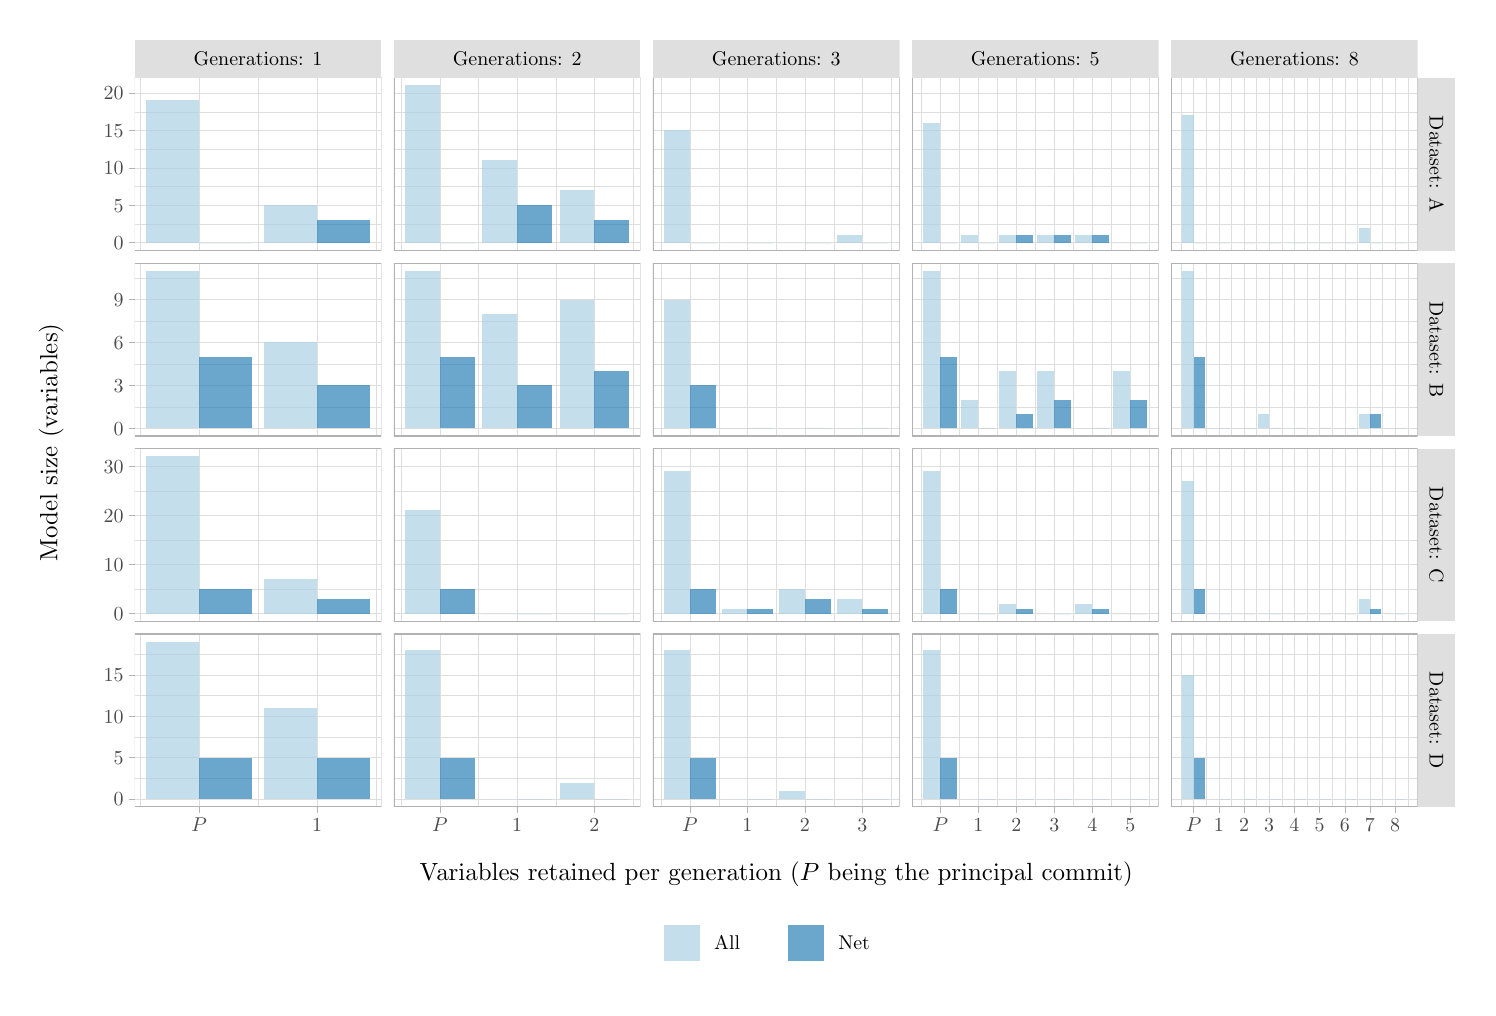
\begin{tikzpicture}[x=1pt,y=1pt]
\definecolor{fillColor}{RGB}{255,255,255}
\path[use as bounding box,fill=fillColor,fill opacity=0.00] (0,0) rectangle (520.34,346.90);
\begin{scope}
\path[clip] (  0.00,  0.00) rectangle (520.34,346.90);
\definecolor{drawColor}{RGB}{255,255,255}
\definecolor{fillColor}{RGB}{255,255,255}

\path[draw=drawColor,line width= 0.5pt,line join=round,line cap=round,fill=fillColor] ( -0.00,  0.00) rectangle (520.34,346.90);
\end{scope}
\begin{scope}
\path[clip] ( 38.70,266.33) rectangle (127.81,328.84);
\definecolor{fillColor}{RGB}{255,255,255}

\path[fill=fillColor] ( 38.70,266.33) rectangle (127.81,328.84);
\definecolor{drawColor}{gray}{0.87}

\path[draw=drawColor,line width= 0.1pt,line join=round] ( 38.70,275.94) --
	(127.81,275.94);

\path[draw=drawColor,line width= 0.1pt,line join=round] ( 38.70,289.47) --
	(127.81,289.47);

\path[draw=drawColor,line width= 0.1pt,line join=round] ( 38.70,303.00) --
	(127.81,303.00);

\path[draw=drawColor,line width= 0.1pt,line join=round] ( 38.70,316.53) --
	(127.81,316.53);

\path[draw=drawColor,line width= 0.1pt,line join=round] ( 40.62,266.33) --
	( 40.62,328.84);

\path[draw=drawColor,line width= 0.1pt,line join=round] ( 83.26,266.33) --
	( 83.26,328.84);

\path[draw=drawColor,line width= 0.1pt,line join=round] (125.90,266.33) --
	(125.90,328.84);

\path[draw=drawColor,line width= 0.2pt,line join=round] ( 38.70,269.17) --
	(127.81,269.17);

\path[draw=drawColor,line width= 0.2pt,line join=round] ( 38.70,282.70) --
	(127.81,282.70);

\path[draw=drawColor,line width= 0.2pt,line join=round] ( 38.70,296.23) --
	(127.81,296.23);

\path[draw=drawColor,line width= 0.2pt,line join=round] ( 38.70,309.76) --
	(127.81,309.76);

\path[draw=drawColor,line width= 0.2pt,line join=round] ( 38.70,323.29) --
	(127.81,323.29);

\path[draw=drawColor,line width= 0.2pt,line join=round] ( 61.94,266.33) --
	( 61.94,328.84);

\path[draw=drawColor,line width= 0.2pt,line join=round] (104.58,266.33) --
	(104.58,328.84);
\definecolor{fillColor}{RGB}{31,120,180}

\path[fill=fillColor,fill opacity=0.66] ( 61.94,269.17) rectangle ( 81.12,269.17);
\definecolor{fillColor}{RGB}{166,206,227}

\path[fill=fillColor,fill opacity=0.66] ( 42.75,269.17) rectangle ( 61.94,320.58);
\definecolor{fillColor}{RGB}{31,120,180}

\path[fill=fillColor,fill opacity=0.66] (104.58,269.17) rectangle (123.76,277.29);
\definecolor{fillColor}{RGB}{166,206,227}

\path[fill=fillColor,fill opacity=0.66] ( 85.39,269.17) rectangle (104.58,282.70);
\definecolor{drawColor}{gray}{0.70}

\path[draw=drawColor,line width= 0.5pt,line join=round,line cap=round] ( 38.70,266.33) rectangle (127.81,328.84);
\end{scope}
\begin{scope}
\path[clip] ( 38.70,199.32) rectangle (127.81,261.83);
\definecolor{fillColor}{RGB}{255,255,255}

\path[fill=fillColor] ( 38.70,199.32) rectangle (127.81,261.83);
\definecolor{drawColor}{gray}{0.87}

\path[draw=drawColor,line width= 0.1pt,line join=round] ( 38.70,209.91) --
	(127.81,209.91);

\path[draw=drawColor,line width= 0.1pt,line join=round] ( 38.70,225.41) --
	(127.81,225.41);

\path[draw=drawColor,line width= 0.1pt,line join=round] ( 38.70,240.91) --
	(127.81,240.91);

\path[draw=drawColor,line width= 0.1pt,line join=round] ( 38.70,256.41) --
	(127.81,256.41);

\path[draw=drawColor,line width= 0.1pt,line join=round] ( 40.62,199.32) --
	( 40.62,261.83);

\path[draw=drawColor,line width= 0.1pt,line join=round] ( 83.26,199.32) --
	( 83.26,261.83);

\path[draw=drawColor,line width= 0.1pt,line join=round] (125.90,199.32) --
	(125.90,261.83);

\path[draw=drawColor,line width= 0.2pt,line join=round] ( 38.70,202.17) --
	(127.81,202.17);

\path[draw=drawColor,line width= 0.2pt,line join=round] ( 38.70,217.66) --
	(127.81,217.66);

\path[draw=drawColor,line width= 0.2pt,line join=round] ( 38.70,233.16) --
	(127.81,233.16);

\path[draw=drawColor,line width= 0.2pt,line join=round] ( 38.70,248.66) --
	(127.81,248.66);

\path[draw=drawColor,line width= 0.2pt,line join=round] ( 61.94,199.32) --
	( 61.94,261.83);

\path[draw=drawColor,line width= 0.2pt,line join=round] (104.58,199.32) --
	(104.58,261.83);
\definecolor{fillColor}{RGB}{31,120,180}

\path[fill=fillColor,fill opacity=0.66] ( 61.94,202.17) rectangle ( 81.12,227.99);
\definecolor{fillColor}{RGB}{166,206,227}

\path[fill=fillColor,fill opacity=0.66] ( 42.75,202.17) rectangle ( 61.94,258.99);
\definecolor{fillColor}{RGB}{31,120,180}

\path[fill=fillColor,fill opacity=0.66] (104.58,202.17) rectangle (123.76,217.66);
\definecolor{fillColor}{RGB}{166,206,227}

\path[fill=fillColor,fill opacity=0.66] ( 85.39,202.17) rectangle (104.58,233.16);
\definecolor{drawColor}{gray}{0.70}

\path[draw=drawColor,line width= 0.5pt,line join=round,line cap=round] ( 38.70,199.32) rectangle (127.81,261.83);
\end{scope}
\begin{scope}
\path[clip] ( 38.70,132.32) rectangle (127.81,194.82);
\definecolor{fillColor}{RGB}{255,255,255}

\path[fill=fillColor] ( 38.70,132.32) rectangle (127.81,194.82);
\definecolor{drawColor}{gray}{0.87}

\path[draw=drawColor,line width= 0.1pt,line join=round] ( 38.70,144.04) --
	(127.81,144.04);

\path[draw=drawColor,line width= 0.1pt,line join=round] ( 38.70,161.79) --
	(127.81,161.79);

\path[draw=drawColor,line width= 0.1pt,line join=round] ( 38.70,179.55) --
	(127.81,179.55);

\path[draw=drawColor,line width= 0.1pt,line join=round] ( 40.62,132.32) --
	( 40.62,194.82);

\path[draw=drawColor,line width= 0.1pt,line join=round] ( 83.26,132.32) --
	( 83.26,194.82);

\path[draw=drawColor,line width= 0.1pt,line join=round] (125.90,132.32) --
	(125.90,194.82);

\path[draw=drawColor,line width= 0.2pt,line join=round] ( 38.70,135.16) --
	(127.81,135.16);

\path[draw=drawColor,line width= 0.2pt,line join=round] ( 38.70,152.92) --
	(127.81,152.92);

\path[draw=drawColor,line width= 0.2pt,line join=round] ( 38.70,170.67) --
	(127.81,170.67);

\path[draw=drawColor,line width= 0.2pt,line join=round] ( 38.70,188.43) --
	(127.81,188.43);

\path[draw=drawColor,line width= 0.2pt,line join=round] ( 61.94,132.32) --
	( 61.94,194.82);

\path[draw=drawColor,line width= 0.2pt,line join=round] (104.58,132.32) --
	(104.58,194.82);
\definecolor{fillColor}{RGB}{31,120,180}

\path[fill=fillColor,fill opacity=0.66] ( 61.94,135.16) rectangle ( 81.12,144.04);
\definecolor{fillColor}{RGB}{166,206,227}

\path[fill=fillColor,fill opacity=0.66] ( 42.75,135.16) rectangle ( 61.94,191.98);
\definecolor{fillColor}{RGB}{31,120,180}

\path[fill=fillColor,fill opacity=0.66] (104.58,135.16) rectangle (123.76,140.49);
\definecolor{fillColor}{RGB}{166,206,227}

\path[fill=fillColor,fill opacity=0.66] ( 85.39,135.16) rectangle (104.58,147.59);
\definecolor{drawColor}{gray}{0.70}

\path[draw=drawColor,line width= 0.5pt,line join=round,line cap=round] ( 38.70,132.32) rectangle (127.81,194.82);
\end{scope}
\begin{scope}
\path[clip] ( 38.70, 65.31) rectangle (127.81,127.82);
\definecolor{fillColor}{RGB}{255,255,255}

\path[fill=fillColor] ( 38.70, 65.31) rectangle (127.81,127.82);
\definecolor{drawColor}{gray}{0.87}

\path[draw=drawColor,line width= 0.1pt,line join=round] ( 38.70, 75.63) --
	(127.81, 75.63);

\path[draw=drawColor,line width= 0.1pt,line join=round] ( 38.70, 90.58) --
	(127.81, 90.58);

\path[draw=drawColor,line width= 0.1pt,line join=round] ( 38.70,105.54) --
	(127.81,105.54);

\path[draw=drawColor,line width= 0.1pt,line join=round] ( 38.70,120.49) --
	(127.81,120.49);

\path[draw=drawColor,line width= 0.1pt,line join=round] ( 40.62, 65.31) --
	( 40.62,127.82);

\path[draw=drawColor,line width= 0.1pt,line join=round] ( 83.26, 65.31) --
	( 83.26,127.82);

\path[draw=drawColor,line width= 0.1pt,line join=round] (125.90, 65.31) --
	(125.90,127.82);

\path[draw=drawColor,line width= 0.2pt,line join=round] ( 38.70, 68.15) --
	(127.81, 68.15);

\path[draw=drawColor,line width= 0.2pt,line join=round] ( 38.70, 83.11) --
	(127.81, 83.11);

\path[draw=drawColor,line width= 0.2pt,line join=round] ( 38.70, 98.06) --
	(127.81, 98.06);

\path[draw=drawColor,line width= 0.2pt,line join=round] ( 38.70,113.01) --
	(127.81,113.01);

\path[draw=drawColor,line width= 0.2pt,line join=round] ( 61.94, 65.31) --
	( 61.94,127.82);

\path[draw=drawColor,line width= 0.2pt,line join=round] (104.58, 65.31) --
	(104.58,127.82);
\definecolor{fillColor}{RGB}{31,120,180}

\path[fill=fillColor,fill opacity=0.66] ( 61.94, 68.15) rectangle ( 81.12, 83.11);
\definecolor{fillColor}{RGB}{166,206,227}

\path[fill=fillColor,fill opacity=0.66] ( 42.75, 68.15) rectangle ( 61.94,124.98);
\definecolor{fillColor}{RGB}{31,120,180}

\path[fill=fillColor,fill opacity=0.66] (104.58, 68.15) rectangle (123.76, 83.11);
\definecolor{fillColor}{RGB}{166,206,227}

\path[fill=fillColor,fill opacity=0.66] ( 85.39, 68.15) rectangle (104.58,101.05);
\definecolor{drawColor}{gray}{0.70}

\path[draw=drawColor,line width= 0.5pt,line join=round,line cap=round] ( 38.70, 65.31) rectangle (127.81,127.82);
\end{scope}
\begin{scope}
\path[clip] (132.31,266.33) rectangle (221.43,328.84);
\definecolor{fillColor}{RGB}{255,255,255}

\path[fill=fillColor] (132.31,266.33) rectangle (221.43,328.84);
\definecolor{drawColor}{gray}{0.87}

\path[draw=drawColor,line width= 0.1pt,line join=round] (132.31,275.94) --
	(221.43,275.94);

\path[draw=drawColor,line width= 0.1pt,line join=round] (132.31,289.47) --
	(221.43,289.47);

\path[draw=drawColor,line width= 0.1pt,line join=round] (132.31,303.00) --
	(221.43,303.00);

\path[draw=drawColor,line width= 0.1pt,line join=round] (132.31,316.53) --
	(221.43,316.53);

\path[draw=drawColor,line width= 0.1pt,line join=round] (134.97,266.33) --
	(134.97,328.84);

\path[draw=drawColor,line width= 0.1pt,line join=round] (162.90,266.33) --
	(162.90,328.84);

\path[draw=drawColor,line width= 0.1pt,line join=round] (190.84,266.33) --
	(190.84,328.84);

\path[draw=drawColor,line width= 0.1pt,line join=round] (218.78,266.33) --
	(218.78,328.84);

\path[draw=drawColor,line width= 0.2pt,line join=round] (132.31,269.17) --
	(221.43,269.17);

\path[draw=drawColor,line width= 0.2pt,line join=round] (132.31,282.70) --
	(221.43,282.70);

\path[draw=drawColor,line width= 0.2pt,line join=round] (132.31,296.23) --
	(221.43,296.23);

\path[draw=drawColor,line width= 0.2pt,line join=round] (132.31,309.76) --
	(221.43,309.76);

\path[draw=drawColor,line width= 0.2pt,line join=round] (132.31,323.29) --
	(221.43,323.29);

\path[draw=drawColor,line width= 0.2pt,line join=round] (148.94,266.33) --
	(148.94,328.84);

\path[draw=drawColor,line width= 0.2pt,line join=round] (176.87,266.33) --
	(176.87,328.84);

\path[draw=drawColor,line width= 0.2pt,line join=round] (204.81,266.33) --
	(204.81,328.84);
\definecolor{fillColor}{RGB}{31,120,180}

\path[fill=fillColor,fill opacity=0.66] (148.94,269.17) rectangle (161.51,269.17);
\definecolor{fillColor}{RGB}{166,206,227}

\path[fill=fillColor,fill opacity=0.66] (136.36,269.17) rectangle (148.94,326.00);
\definecolor{fillColor}{RGB}{31,120,180}

\path[fill=fillColor,fill opacity=0.66] (176.87,269.17) rectangle (189.44,282.70);
\definecolor{fillColor}{RGB}{166,206,227}

\path[fill=fillColor,fill opacity=0.66] (164.30,269.17) rectangle (176.87,298.94);
\definecolor{fillColor}{RGB}{31,120,180}

\path[fill=fillColor,fill opacity=0.66] (204.81,269.17) rectangle (217.38,277.29);
\definecolor{fillColor}{RGB}{166,206,227}

\path[fill=fillColor,fill opacity=0.66] (192.24,269.17) rectangle (204.81,288.11);
\definecolor{drawColor}{gray}{0.70}

\path[draw=drawColor,line width= 0.5pt,line join=round,line cap=round] (132.31,266.33) rectangle (221.43,328.84);
\end{scope}
\begin{scope}
\path[clip] (132.31,199.32) rectangle (221.43,261.83);
\definecolor{fillColor}{RGB}{255,255,255}

\path[fill=fillColor] (132.31,199.32) rectangle (221.43,261.83);
\definecolor{drawColor}{gray}{0.87}

\path[draw=drawColor,line width= 0.1pt,line join=round] (132.31,209.91) --
	(221.43,209.91);

\path[draw=drawColor,line width= 0.1pt,line join=round] (132.31,225.41) --
	(221.43,225.41);

\path[draw=drawColor,line width= 0.1pt,line join=round] (132.31,240.91) --
	(221.43,240.91);

\path[draw=drawColor,line width= 0.1pt,line join=round] (132.31,256.41) --
	(221.43,256.41);

\path[draw=drawColor,line width= 0.1pt,line join=round] (134.97,199.32) --
	(134.97,261.83);

\path[draw=drawColor,line width= 0.1pt,line join=round] (162.90,199.32) --
	(162.90,261.83);

\path[draw=drawColor,line width= 0.1pt,line join=round] (190.84,199.32) --
	(190.84,261.83);

\path[draw=drawColor,line width= 0.1pt,line join=round] (218.78,199.32) --
	(218.78,261.83);

\path[draw=drawColor,line width= 0.2pt,line join=round] (132.31,202.17) --
	(221.43,202.17);

\path[draw=drawColor,line width= 0.2pt,line join=round] (132.31,217.66) --
	(221.43,217.66);

\path[draw=drawColor,line width= 0.2pt,line join=round] (132.31,233.16) --
	(221.43,233.16);

\path[draw=drawColor,line width= 0.2pt,line join=round] (132.31,248.66) --
	(221.43,248.66);

\path[draw=drawColor,line width= 0.2pt,line join=round] (148.94,199.32) --
	(148.94,261.83);

\path[draw=drawColor,line width= 0.2pt,line join=round] (176.87,199.32) --
	(176.87,261.83);

\path[draw=drawColor,line width= 0.2pt,line join=round] (204.81,199.32) --
	(204.81,261.83);
\definecolor{fillColor}{RGB}{31,120,180}

\path[fill=fillColor,fill opacity=0.66] (148.94,202.17) rectangle (161.51,227.99);
\definecolor{fillColor}{RGB}{166,206,227}

\path[fill=fillColor,fill opacity=0.66] (136.36,202.17) rectangle (148.94,258.99);
\definecolor{fillColor}{RGB}{31,120,180}

\path[fill=fillColor,fill opacity=0.66] (176.87,202.17) rectangle (189.44,217.66);
\definecolor{fillColor}{RGB}{166,206,227}

\path[fill=fillColor,fill opacity=0.66] (164.30,202.17) rectangle (176.87,243.49);
\definecolor{fillColor}{RGB}{31,120,180}

\path[fill=fillColor,fill opacity=0.66] (204.81,202.17) rectangle (217.38,222.83);
\definecolor{fillColor}{RGB}{166,206,227}

\path[fill=fillColor,fill opacity=0.66] (192.24,202.17) rectangle (204.81,248.66);
\definecolor{drawColor}{gray}{0.70}

\path[draw=drawColor,line width= 0.5pt,line join=round,line cap=round] (132.31,199.32) rectangle (221.43,261.83);
\end{scope}
\begin{scope}
\path[clip] (132.31,132.32) rectangle (221.43,194.82);
\definecolor{fillColor}{RGB}{255,255,255}

\path[fill=fillColor] (132.31,132.32) rectangle (221.43,194.82);
\definecolor{drawColor}{gray}{0.87}

\path[draw=drawColor,line width= 0.1pt,line join=round] (132.31,144.04) --
	(221.43,144.04);

\path[draw=drawColor,line width= 0.1pt,line join=round] (132.31,161.79) --
	(221.43,161.79);

\path[draw=drawColor,line width= 0.1pt,line join=round] (132.31,179.55) --
	(221.43,179.55);

\path[draw=drawColor,line width= 0.1pt,line join=round] (134.97,132.32) --
	(134.97,194.82);

\path[draw=drawColor,line width= 0.1pt,line join=round] (162.90,132.32) --
	(162.90,194.82);

\path[draw=drawColor,line width= 0.1pt,line join=round] (190.84,132.32) --
	(190.84,194.82);

\path[draw=drawColor,line width= 0.1pt,line join=round] (218.78,132.32) --
	(218.78,194.82);

\path[draw=drawColor,line width= 0.2pt,line join=round] (132.31,135.16) --
	(221.43,135.16);

\path[draw=drawColor,line width= 0.2pt,line join=round] (132.31,152.92) --
	(221.43,152.92);

\path[draw=drawColor,line width= 0.2pt,line join=round] (132.31,170.67) --
	(221.43,170.67);

\path[draw=drawColor,line width= 0.2pt,line join=round] (132.31,188.43) --
	(221.43,188.43);

\path[draw=drawColor,line width= 0.2pt,line join=round] (148.94,132.32) --
	(148.94,194.82);

\path[draw=drawColor,line width= 0.2pt,line join=round] (176.87,132.32) --
	(176.87,194.82);

\path[draw=drawColor,line width= 0.2pt,line join=round] (204.81,132.32) --
	(204.81,194.82);
\definecolor{fillColor}{RGB}{31,120,180}

\path[fill=fillColor,fill opacity=0.66] (148.94,135.16) rectangle (161.51,144.04);
\definecolor{fillColor}{RGB}{166,206,227}

\path[fill=fillColor,fill opacity=0.66] (136.36,135.16) rectangle (148.94,172.45);
\definecolor{fillColor}{RGB}{31,120,180}

\path[fill=fillColor,fill opacity=0.66] (176.87,135.16) rectangle (189.44,135.16);
\definecolor{fillColor}{RGB}{166,206,227}

\path[fill=fillColor,fill opacity=0.66] (164.30,135.16) rectangle (176.87,135.16);
\definecolor{fillColor}{RGB}{31,120,180}

\path[fill=fillColor,fill opacity=0.66] (204.81,135.16) rectangle (217.38,135.16);
\definecolor{fillColor}{RGB}{166,206,227}

\path[fill=fillColor,fill opacity=0.66] (192.24,135.16) rectangle (204.81,135.16);
\definecolor{drawColor}{gray}{0.70}

\path[draw=drawColor,line width= 0.5pt,line join=round,line cap=round] (132.31,132.32) rectangle (221.43,194.82);
\end{scope}
\begin{scope}
\path[clip] (132.31, 65.31) rectangle (221.43,127.82);
\definecolor{fillColor}{RGB}{255,255,255}

\path[fill=fillColor] (132.31, 65.31) rectangle (221.43,127.82);
\definecolor{drawColor}{gray}{0.87}

\path[draw=drawColor,line width= 0.1pt,line join=round] (132.31, 75.63) --
	(221.43, 75.63);

\path[draw=drawColor,line width= 0.1pt,line join=round] (132.31, 90.58) --
	(221.43, 90.58);

\path[draw=drawColor,line width= 0.1pt,line join=round] (132.31,105.54) --
	(221.43,105.54);

\path[draw=drawColor,line width= 0.1pt,line join=round] (132.31,120.49) --
	(221.43,120.49);

\path[draw=drawColor,line width= 0.1pt,line join=round] (134.97, 65.31) --
	(134.97,127.82);

\path[draw=drawColor,line width= 0.1pt,line join=round] (162.90, 65.31) --
	(162.90,127.82);

\path[draw=drawColor,line width= 0.1pt,line join=round] (190.84, 65.31) --
	(190.84,127.82);

\path[draw=drawColor,line width= 0.1pt,line join=round] (218.78, 65.31) --
	(218.78,127.82);

\path[draw=drawColor,line width= 0.2pt,line join=round] (132.31, 68.15) --
	(221.43, 68.15);

\path[draw=drawColor,line width= 0.2pt,line join=round] (132.31, 83.11) --
	(221.43, 83.11);

\path[draw=drawColor,line width= 0.2pt,line join=round] (132.31, 98.06) --
	(221.43, 98.06);

\path[draw=drawColor,line width= 0.2pt,line join=round] (132.31,113.01) --
	(221.43,113.01);

\path[draw=drawColor,line width= 0.2pt,line join=round] (148.94, 65.31) --
	(148.94,127.82);

\path[draw=drawColor,line width= 0.2pt,line join=round] (176.87, 65.31) --
	(176.87,127.82);

\path[draw=drawColor,line width= 0.2pt,line join=round] (204.81, 65.31) --
	(204.81,127.82);
\definecolor{fillColor}{RGB}{31,120,180}

\path[fill=fillColor,fill opacity=0.66] (148.94, 68.15) rectangle (161.51, 83.11);
\definecolor{fillColor}{RGB}{166,206,227}

\path[fill=fillColor,fill opacity=0.66] (136.36, 68.15) rectangle (148.94,121.99);
\definecolor{fillColor}{RGB}{31,120,180}

\path[fill=fillColor,fill opacity=0.66] (176.87, 68.15) rectangle (189.44, 68.15);
\definecolor{fillColor}{RGB}{166,206,227}

\path[fill=fillColor,fill opacity=0.66] (164.30, 68.15) rectangle (176.87, 68.15);
\definecolor{fillColor}{RGB}{31,120,180}

\path[fill=fillColor,fill opacity=0.66] (204.81, 68.15) rectangle (217.38, 68.15);
\definecolor{fillColor}{RGB}{166,206,227}

\path[fill=fillColor,fill opacity=0.66] (192.24, 68.15) rectangle (204.81, 74.13);
\definecolor{drawColor}{gray}{0.70}

\path[draw=drawColor,line width= 0.5pt,line join=round,line cap=round] (132.31, 65.31) rectangle (221.43,127.82);
\end{scope}
\begin{scope}
\path[clip] (225.93,266.33) rectangle (315.05,328.84);
\definecolor{fillColor}{RGB}{255,255,255}

\path[fill=fillColor] (225.93,266.33) rectangle (315.05,328.84);
\definecolor{drawColor}{gray}{0.87}

\path[draw=drawColor,line width= 0.1pt,line join=round] (225.93,275.94) --
	(315.05,275.94);

\path[draw=drawColor,line width= 0.1pt,line join=round] (225.93,289.47) --
	(315.05,289.47);

\path[draw=drawColor,line width= 0.1pt,line join=round] (225.93,303.00) --
	(315.05,303.00);

\path[draw=drawColor,line width= 0.1pt,line join=round] (225.93,316.53) --
	(315.05,316.53);

\path[draw=drawColor,line width= 0.1pt,line join=round] (228.94,266.33) --
	(228.94,328.84);

\path[draw=drawColor,line width= 0.1pt,line join=round] (249.72,266.33) --
	(249.72,328.84);

\path[draw=drawColor,line width= 0.1pt,line join=round] (270.49,266.33) --
	(270.49,328.84);

\path[draw=drawColor,line width= 0.1pt,line join=round] (291.26,266.33) --
	(291.26,328.84);

\path[draw=drawColor,line width= 0.1pt,line join=round] (312.04,266.33) --
	(312.04,328.84);

\path[draw=drawColor,line width= 0.2pt,line join=round] (225.93,269.17) --
	(315.05,269.17);

\path[draw=drawColor,line width= 0.2pt,line join=round] (225.93,282.70) --
	(315.05,282.70);

\path[draw=drawColor,line width= 0.2pt,line join=round] (225.93,296.23) --
	(315.05,296.23);

\path[draw=drawColor,line width= 0.2pt,line join=round] (225.93,309.76) --
	(315.05,309.76);

\path[draw=drawColor,line width= 0.2pt,line join=round] (225.93,323.29) --
	(315.05,323.29);

\path[draw=drawColor,line width= 0.2pt,line join=round] (239.33,266.33) --
	(239.33,328.84);

\path[draw=drawColor,line width= 0.2pt,line join=round] (260.10,266.33) --
	(260.10,328.84);

\path[draw=drawColor,line width= 0.2pt,line join=round] (280.88,266.33) --
	(280.88,328.84);

\path[draw=drawColor,line width= 0.2pt,line join=round] (301.65,266.33) --
	(301.65,328.84);
\definecolor{fillColor}{RGB}{31,120,180}

\path[fill=fillColor,fill opacity=0.66] (239.33,269.17) rectangle (248.68,269.17);
\definecolor{fillColor}{RGB}{166,206,227}

\path[fill=fillColor,fill opacity=0.66] (229.98,269.17) rectangle (239.33,309.76);
\definecolor{fillColor}{RGB}{31,120,180}

\path[fill=fillColor,fill opacity=0.66] (260.10,269.17) rectangle (269.45,269.17);
\definecolor{fillColor}{RGB}{166,206,227}

\path[fill=fillColor,fill opacity=0.66] (250.76,269.17) rectangle (260.10,269.17);
\definecolor{fillColor}{RGB}{31,120,180}

\path[fill=fillColor,fill opacity=0.66] (280.88,269.17) rectangle (290.23,269.17);
\definecolor{fillColor}{RGB}{166,206,227}

\path[fill=fillColor,fill opacity=0.66] (271.53,269.17) rectangle (280.88,269.17);
\definecolor{fillColor}{RGB}{31,120,180}

\path[fill=fillColor,fill opacity=0.66] (301.65,269.17) rectangle (311.00,269.17);
\definecolor{fillColor}{RGB}{166,206,227}

\path[fill=fillColor,fill opacity=0.66] (292.30,269.17) rectangle (301.65,271.88);
\definecolor{drawColor}{gray}{0.70}

\path[draw=drawColor,line width= 0.5pt,line join=round,line cap=round] (225.93,266.33) rectangle (315.05,328.84);
\end{scope}
\begin{scope}
\path[clip] (225.93,199.32) rectangle (315.05,261.83);
\definecolor{fillColor}{RGB}{255,255,255}

\path[fill=fillColor] (225.93,199.32) rectangle (315.05,261.83);
\definecolor{drawColor}{gray}{0.87}

\path[draw=drawColor,line width= 0.1pt,line join=round] (225.93,209.91) --
	(315.05,209.91);

\path[draw=drawColor,line width= 0.1pt,line join=round] (225.93,225.41) --
	(315.05,225.41);

\path[draw=drawColor,line width= 0.1pt,line join=round] (225.93,240.91) --
	(315.05,240.91);

\path[draw=drawColor,line width= 0.1pt,line join=round] (225.93,256.41) --
	(315.05,256.41);

\path[draw=drawColor,line width= 0.1pt,line join=round] (228.94,199.32) --
	(228.94,261.83);

\path[draw=drawColor,line width= 0.1pt,line join=round] (249.72,199.32) --
	(249.72,261.83);

\path[draw=drawColor,line width= 0.1pt,line join=round] (270.49,199.32) --
	(270.49,261.83);

\path[draw=drawColor,line width= 0.1pt,line join=round] (291.26,199.32) --
	(291.26,261.83);

\path[draw=drawColor,line width= 0.1pt,line join=round] (312.04,199.32) --
	(312.04,261.83);

\path[draw=drawColor,line width= 0.2pt,line join=round] (225.93,202.17) --
	(315.05,202.17);

\path[draw=drawColor,line width= 0.2pt,line join=round] (225.93,217.66) --
	(315.05,217.66);

\path[draw=drawColor,line width= 0.2pt,line join=round] (225.93,233.16) --
	(315.05,233.16);

\path[draw=drawColor,line width= 0.2pt,line join=round] (225.93,248.66) --
	(315.05,248.66);

\path[draw=drawColor,line width= 0.2pt,line join=round] (239.33,199.32) --
	(239.33,261.83);

\path[draw=drawColor,line width= 0.2pt,line join=round] (260.10,199.32) --
	(260.10,261.83);

\path[draw=drawColor,line width= 0.2pt,line join=round] (280.88,199.32) --
	(280.88,261.83);

\path[draw=drawColor,line width= 0.2pt,line join=round] (301.65,199.32) --
	(301.65,261.83);
\definecolor{fillColor}{RGB}{31,120,180}

\path[fill=fillColor,fill opacity=0.66] (239.33,202.17) rectangle (248.68,217.66);
\definecolor{fillColor}{RGB}{166,206,227}

\path[fill=fillColor,fill opacity=0.66] (229.98,202.17) rectangle (239.33,248.66);
\definecolor{fillColor}{RGB}{31,120,180}

\path[fill=fillColor,fill opacity=0.66] (260.10,202.17) rectangle (269.45,202.17);
\definecolor{fillColor}{RGB}{166,206,227}

\path[fill=fillColor,fill opacity=0.66] (250.76,202.17) rectangle (260.10,202.17);
\definecolor{fillColor}{RGB}{31,120,180}

\path[fill=fillColor,fill opacity=0.66] (280.88,202.17) rectangle (290.23,202.17);
\definecolor{fillColor}{RGB}{166,206,227}

\path[fill=fillColor,fill opacity=0.66] (271.53,202.17) rectangle (280.88,202.17);
\definecolor{fillColor}{RGB}{31,120,180}

\path[fill=fillColor,fill opacity=0.66] (301.65,202.17) rectangle (311.00,202.17);
\definecolor{fillColor}{RGB}{166,206,227}

\path[fill=fillColor,fill opacity=0.66] (292.30,202.17) rectangle (301.65,202.17);
\definecolor{drawColor}{gray}{0.70}

\path[draw=drawColor,line width= 0.5pt,line join=round,line cap=round] (225.93,199.32) rectangle (315.05,261.83);
\end{scope}
\begin{scope}
\path[clip] (225.93,132.32) rectangle (315.05,194.82);
\definecolor{fillColor}{RGB}{255,255,255}

\path[fill=fillColor] (225.93,132.32) rectangle (315.05,194.82);
\definecolor{drawColor}{gray}{0.87}

\path[draw=drawColor,line width= 0.1pt,line join=round] (225.93,144.04) --
	(315.05,144.04);

\path[draw=drawColor,line width= 0.1pt,line join=round] (225.93,161.79) --
	(315.05,161.79);

\path[draw=drawColor,line width= 0.1pt,line join=round] (225.93,179.55) --
	(315.05,179.55);

\path[draw=drawColor,line width= 0.1pt,line join=round] (228.94,132.32) --
	(228.94,194.82);

\path[draw=drawColor,line width= 0.1pt,line join=round] (249.72,132.32) --
	(249.72,194.82);

\path[draw=drawColor,line width= 0.1pt,line join=round] (270.49,132.32) --
	(270.49,194.82);

\path[draw=drawColor,line width= 0.1pt,line join=round] (291.26,132.32) --
	(291.26,194.82);

\path[draw=drawColor,line width= 0.1pt,line join=round] (312.04,132.32) --
	(312.04,194.82);

\path[draw=drawColor,line width= 0.2pt,line join=round] (225.93,135.16) --
	(315.05,135.16);

\path[draw=drawColor,line width= 0.2pt,line join=round] (225.93,152.92) --
	(315.05,152.92);

\path[draw=drawColor,line width= 0.2pt,line join=round] (225.93,170.67) --
	(315.05,170.67);

\path[draw=drawColor,line width= 0.2pt,line join=round] (225.93,188.43) --
	(315.05,188.43);

\path[draw=drawColor,line width= 0.2pt,line join=round] (239.33,132.32) --
	(239.33,194.82);

\path[draw=drawColor,line width= 0.2pt,line join=round] (260.10,132.32) --
	(260.10,194.82);

\path[draw=drawColor,line width= 0.2pt,line join=round] (280.88,132.32) --
	(280.88,194.82);

\path[draw=drawColor,line width= 0.2pt,line join=round] (301.65,132.32) --
	(301.65,194.82);
\definecolor{fillColor}{RGB}{31,120,180}

\path[fill=fillColor,fill opacity=0.66] (239.33,135.16) rectangle (248.68,144.04);
\definecolor{fillColor}{RGB}{166,206,227}

\path[fill=fillColor,fill opacity=0.66] (229.98,135.16) rectangle (239.33,186.66);
\definecolor{fillColor}{RGB}{31,120,180}

\path[fill=fillColor,fill opacity=0.66] (260.10,135.16) rectangle (269.45,136.93);
\definecolor{fillColor}{RGB}{166,206,227}

\path[fill=fillColor,fill opacity=0.66] (250.76,135.16) rectangle (260.10,136.93);
\definecolor{fillColor}{RGB}{31,120,180}

\path[fill=fillColor,fill opacity=0.66] (280.88,135.16) rectangle (290.23,140.49);
\definecolor{fillColor}{RGB}{166,206,227}

\path[fill=fillColor,fill opacity=0.66] (271.53,135.16) rectangle (280.88,144.04);
\definecolor{fillColor}{RGB}{31,120,180}

\path[fill=fillColor,fill opacity=0.66] (301.65,135.16) rectangle (311.00,136.93);
\definecolor{fillColor}{RGB}{166,206,227}

\path[fill=fillColor,fill opacity=0.66] (292.30,135.16) rectangle (301.65,140.49);
\definecolor{drawColor}{gray}{0.70}

\path[draw=drawColor,line width= 0.5pt,line join=round,line cap=round] (225.93,132.32) rectangle (315.05,194.82);
\end{scope}
\begin{scope}
\path[clip] (225.93, 65.31) rectangle (315.05,127.82);
\definecolor{fillColor}{RGB}{255,255,255}

\path[fill=fillColor] (225.93, 65.31) rectangle (315.05,127.82);
\definecolor{drawColor}{gray}{0.87}

\path[draw=drawColor,line width= 0.1pt,line join=round] (225.93, 75.63) --
	(315.05, 75.63);

\path[draw=drawColor,line width= 0.1pt,line join=round] (225.93, 90.58) --
	(315.05, 90.58);

\path[draw=drawColor,line width= 0.1pt,line join=round] (225.93,105.54) --
	(315.05,105.54);

\path[draw=drawColor,line width= 0.1pt,line join=round] (225.93,120.49) --
	(315.05,120.49);

\path[draw=drawColor,line width= 0.1pt,line join=round] (228.94, 65.31) --
	(228.94,127.82);

\path[draw=drawColor,line width= 0.1pt,line join=round] (249.72, 65.31) --
	(249.72,127.82);

\path[draw=drawColor,line width= 0.1pt,line join=round] (270.49, 65.31) --
	(270.49,127.82);

\path[draw=drawColor,line width= 0.1pt,line join=round] (291.26, 65.31) --
	(291.26,127.82);

\path[draw=drawColor,line width= 0.1pt,line join=round] (312.04, 65.31) --
	(312.04,127.82);

\path[draw=drawColor,line width= 0.2pt,line join=round] (225.93, 68.15) --
	(315.05, 68.15);

\path[draw=drawColor,line width= 0.2pt,line join=round] (225.93, 83.11) --
	(315.05, 83.11);

\path[draw=drawColor,line width= 0.2pt,line join=round] (225.93, 98.06) --
	(315.05, 98.06);

\path[draw=drawColor,line width= 0.2pt,line join=round] (225.93,113.01) --
	(315.05,113.01);

\path[draw=drawColor,line width= 0.2pt,line join=round] (239.33, 65.31) --
	(239.33,127.82);

\path[draw=drawColor,line width= 0.2pt,line join=round] (260.10, 65.31) --
	(260.10,127.82);

\path[draw=drawColor,line width= 0.2pt,line join=round] (280.88, 65.31) --
	(280.88,127.82);

\path[draw=drawColor,line width= 0.2pt,line join=round] (301.65, 65.31) --
	(301.65,127.82);
\definecolor{fillColor}{RGB}{31,120,180}

\path[fill=fillColor,fill opacity=0.66] (239.33, 68.15) rectangle (248.68, 83.11);
\definecolor{fillColor}{RGB}{166,206,227}

\path[fill=fillColor,fill opacity=0.66] (229.98, 68.15) rectangle (239.33,121.99);
\definecolor{fillColor}{RGB}{31,120,180}

\path[fill=fillColor,fill opacity=0.66] (260.10, 68.15) rectangle (269.45, 68.15);
\definecolor{fillColor}{RGB}{166,206,227}

\path[fill=fillColor,fill opacity=0.66] (250.76, 68.15) rectangle (260.10, 68.15);
\definecolor{fillColor}{RGB}{31,120,180}

\path[fill=fillColor,fill opacity=0.66] (280.88, 68.15) rectangle (290.23, 68.15);
\definecolor{fillColor}{RGB}{166,206,227}

\path[fill=fillColor,fill opacity=0.66] (271.53, 68.15) rectangle (280.88, 71.14);
\definecolor{fillColor}{RGB}{31,120,180}

\path[fill=fillColor,fill opacity=0.66] (301.65, 68.15) rectangle (311.00, 68.15);
\definecolor{fillColor}{RGB}{166,206,227}

\path[fill=fillColor,fill opacity=0.66] (292.30, 68.15) rectangle (301.65, 68.15);
\definecolor{drawColor}{gray}{0.70}

\path[draw=drawColor,line width= 0.5pt,line join=round,line cap=round] (225.93, 65.31) rectangle (315.05,127.82);
\end{scope}
\begin{scope}
\path[clip] (319.55,266.33) rectangle (408.67,328.84);
\definecolor{fillColor}{RGB}{255,255,255}

\path[fill=fillColor] (319.55,266.33) rectangle (408.67,328.84);
\definecolor{drawColor}{gray}{0.87}

\path[draw=drawColor,line width= 0.1pt,line join=round] (319.55,275.94) --
	(408.67,275.94);

\path[draw=drawColor,line width= 0.1pt,line join=round] (319.55,289.47) --
	(408.67,289.47);

\path[draw=drawColor,line width= 0.1pt,line join=round] (319.55,303.00) --
	(408.67,303.00);

\path[draw=drawColor,line width= 0.1pt,line join=round] (319.55,316.53) --
	(408.67,316.53);

\path[draw=drawColor,line width= 0.1pt,line join=round] (322.91,266.33) --
	(322.91,328.84);

\path[draw=drawColor,line width= 0.1pt,line join=round] (336.65,266.33) --
	(336.65,328.84);

\path[draw=drawColor,line width= 0.1pt,line join=round] (350.38,266.33) --
	(350.38,328.84);

\path[draw=drawColor,line width= 0.1pt,line join=round] (364.11,266.33) --
	(364.11,328.84);

\path[draw=drawColor,line width= 0.1pt,line join=round] (377.84,266.33) --
	(377.84,328.84);

\path[draw=drawColor,line width= 0.1pt,line join=round] (391.57,266.33) --
	(391.57,328.84);

\path[draw=drawColor,line width= 0.1pt,line join=round] (405.30,266.33) --
	(405.30,328.84);

\path[draw=drawColor,line width= 0.2pt,line join=round] (319.55,269.17) --
	(408.67,269.17);

\path[draw=drawColor,line width= 0.2pt,line join=round] (319.55,282.70) --
	(408.67,282.70);

\path[draw=drawColor,line width= 0.2pt,line join=round] (319.55,296.23) --
	(408.67,296.23);

\path[draw=drawColor,line width= 0.2pt,line join=round] (319.55,309.76) --
	(408.67,309.76);

\path[draw=drawColor,line width= 0.2pt,line join=round] (319.55,323.29) --
	(408.67,323.29);

\path[draw=drawColor,line width= 0.2pt,line join=round] (329.78,266.33) --
	(329.78,328.84);

\path[draw=drawColor,line width= 0.2pt,line join=round] (343.51,266.33) --
	(343.51,328.84);

\path[draw=drawColor,line width= 0.2pt,line join=round] (357.24,266.33) --
	(357.24,328.84);

\path[draw=drawColor,line width= 0.2pt,line join=round] (370.97,266.33) --
	(370.97,328.84);

\path[draw=drawColor,line width= 0.2pt,line join=round] (384.71,266.33) --
	(384.71,328.84);

\path[draw=drawColor,line width= 0.2pt,line join=round] (398.44,266.33) --
	(398.44,328.84);
\definecolor{fillColor}{RGB}{31,120,180}

\path[fill=fillColor,fill opacity=0.66] (329.78,269.17) rectangle (335.96,269.17);
\definecolor{fillColor}{RGB}{166,206,227}

\path[fill=fillColor,fill opacity=0.66] (323.60,269.17) rectangle (329.78,312.47);
\definecolor{fillColor}{RGB}{31,120,180}

\path[fill=fillColor,fill opacity=0.66] (343.51,269.17) rectangle (349.69,269.17);
\definecolor{fillColor}{RGB}{166,206,227}

\path[fill=fillColor,fill opacity=0.66] (337.33,269.17) rectangle (343.51,271.88);
\definecolor{fillColor}{RGB}{31,120,180}

\path[fill=fillColor,fill opacity=0.66] (357.24,269.17) rectangle (363.42,271.88);
\definecolor{fillColor}{RGB}{166,206,227}

\path[fill=fillColor,fill opacity=0.66] (351.06,269.17) rectangle (357.24,271.88);
\definecolor{fillColor}{RGB}{31,120,180}

\path[fill=fillColor,fill opacity=0.66] (370.97,269.17) rectangle (377.15,271.88);
\definecolor{fillColor}{RGB}{166,206,227}

\path[fill=fillColor,fill opacity=0.66] (364.80,269.17) rectangle (370.97,271.88);
\definecolor{fillColor}{RGB}{31,120,180}

\path[fill=fillColor,fill opacity=0.66] (384.71,269.17) rectangle (390.89,271.88);
\definecolor{fillColor}{RGB}{166,206,227}

\path[fill=fillColor,fill opacity=0.66] (378.53,269.17) rectangle (384.71,271.88);
\definecolor{fillColor}{RGB}{31,120,180}

\path[fill=fillColor,fill opacity=0.66] (398.44,269.17) rectangle (404.62,269.17);
\definecolor{fillColor}{RGB}{166,206,227}

\path[fill=fillColor,fill opacity=0.66] (392.26,269.17) rectangle (398.44,269.17);
\definecolor{drawColor}{gray}{0.70}

\path[draw=drawColor,line width= 0.5pt,line join=round,line cap=round] (319.55,266.33) rectangle (408.67,328.84);
\end{scope}
\begin{scope}
\path[clip] (319.55,199.32) rectangle (408.67,261.83);
\definecolor{fillColor}{RGB}{255,255,255}

\path[fill=fillColor] (319.55,199.32) rectangle (408.67,261.83);
\definecolor{drawColor}{gray}{0.87}

\path[draw=drawColor,line width= 0.1pt,line join=round] (319.55,209.91) --
	(408.67,209.91);

\path[draw=drawColor,line width= 0.1pt,line join=round] (319.55,225.41) --
	(408.67,225.41);

\path[draw=drawColor,line width= 0.1pt,line join=round] (319.55,240.91) --
	(408.67,240.91);

\path[draw=drawColor,line width= 0.1pt,line join=round] (319.55,256.41) --
	(408.67,256.41);

\path[draw=drawColor,line width= 0.1pt,line join=round] (322.91,199.32) --
	(322.91,261.83);

\path[draw=drawColor,line width= 0.1pt,line join=round] (336.65,199.32) --
	(336.65,261.83);

\path[draw=drawColor,line width= 0.1pt,line join=round] (350.38,199.32) --
	(350.38,261.83);

\path[draw=drawColor,line width= 0.1pt,line join=round] (364.11,199.32) --
	(364.11,261.83);

\path[draw=drawColor,line width= 0.1pt,line join=round] (377.84,199.32) --
	(377.84,261.83);

\path[draw=drawColor,line width= 0.1pt,line join=round] (391.57,199.32) --
	(391.57,261.83);

\path[draw=drawColor,line width= 0.1pt,line join=round] (405.30,199.32) --
	(405.30,261.83);

\path[draw=drawColor,line width= 0.2pt,line join=round] (319.55,202.17) --
	(408.67,202.17);

\path[draw=drawColor,line width= 0.2pt,line join=round] (319.55,217.66) --
	(408.67,217.66);

\path[draw=drawColor,line width= 0.2pt,line join=round] (319.55,233.16) --
	(408.67,233.16);

\path[draw=drawColor,line width= 0.2pt,line join=round] (319.55,248.66) --
	(408.67,248.66);

\path[draw=drawColor,line width= 0.2pt,line join=round] (329.78,199.32) --
	(329.78,261.83);

\path[draw=drawColor,line width= 0.2pt,line join=round] (343.51,199.32) --
	(343.51,261.83);

\path[draw=drawColor,line width= 0.2pt,line join=round] (357.24,199.32) --
	(357.24,261.83);

\path[draw=drawColor,line width= 0.2pt,line join=round] (370.97,199.32) --
	(370.97,261.83);

\path[draw=drawColor,line width= 0.2pt,line join=round] (384.71,199.32) --
	(384.71,261.83);

\path[draw=drawColor,line width= 0.2pt,line join=round] (398.44,199.32) --
	(398.44,261.83);
\definecolor{fillColor}{RGB}{31,120,180}

\path[fill=fillColor,fill opacity=0.66] (329.78,202.17) rectangle (335.96,227.99);
\definecolor{fillColor}{RGB}{166,206,227}

\path[fill=fillColor,fill opacity=0.66] (323.60,202.17) rectangle (329.78,258.99);
\definecolor{fillColor}{RGB}{31,120,180}

\path[fill=fillColor,fill opacity=0.66] (343.51,202.17) rectangle (349.69,202.17);
\definecolor{fillColor}{RGB}{166,206,227}

\path[fill=fillColor,fill opacity=0.66] (337.33,202.17) rectangle (343.51,212.50);
\definecolor{fillColor}{RGB}{31,120,180}

\path[fill=fillColor,fill opacity=0.66] (357.24,202.17) rectangle (363.42,207.33);
\definecolor{fillColor}{RGB}{166,206,227}

\path[fill=fillColor,fill opacity=0.66] (351.06,202.17) rectangle (357.24,222.83);
\definecolor{fillColor}{RGB}{31,120,180}

\path[fill=fillColor,fill opacity=0.66] (370.97,202.17) rectangle (377.15,212.50);
\definecolor{fillColor}{RGB}{166,206,227}

\path[fill=fillColor,fill opacity=0.66] (364.80,202.17) rectangle (370.97,222.83);
\definecolor{fillColor}{RGB}{31,120,180}

\path[fill=fillColor,fill opacity=0.66] (384.71,202.17) rectangle (390.89,202.17);
\definecolor{fillColor}{RGB}{166,206,227}

\path[fill=fillColor,fill opacity=0.66] (378.53,202.17) rectangle (384.71,202.17);
\definecolor{fillColor}{RGB}{31,120,180}

\path[fill=fillColor,fill opacity=0.66] (398.44,202.17) rectangle (404.62,212.50);
\definecolor{fillColor}{RGB}{166,206,227}

\path[fill=fillColor,fill opacity=0.66] (392.26,202.17) rectangle (398.44,222.83);
\definecolor{drawColor}{gray}{0.70}

\path[draw=drawColor,line width= 0.5pt,line join=round,line cap=round] (319.55,199.32) rectangle (408.67,261.83);
\end{scope}
\begin{scope}
\path[clip] (319.55,132.32) rectangle (408.67,194.82);
\definecolor{fillColor}{RGB}{255,255,255}

\path[fill=fillColor] (319.55,132.32) rectangle (408.67,194.82);
\definecolor{drawColor}{gray}{0.87}

\path[draw=drawColor,line width= 0.1pt,line join=round] (319.55,144.04) --
	(408.67,144.04);

\path[draw=drawColor,line width= 0.1pt,line join=round] (319.55,161.79) --
	(408.67,161.79);

\path[draw=drawColor,line width= 0.1pt,line join=round] (319.55,179.55) --
	(408.67,179.55);

\path[draw=drawColor,line width= 0.1pt,line join=round] (322.91,132.32) --
	(322.91,194.82);

\path[draw=drawColor,line width= 0.1pt,line join=round] (336.65,132.32) --
	(336.65,194.82);

\path[draw=drawColor,line width= 0.1pt,line join=round] (350.38,132.32) --
	(350.38,194.82);

\path[draw=drawColor,line width= 0.1pt,line join=round] (364.11,132.32) --
	(364.11,194.82);

\path[draw=drawColor,line width= 0.1pt,line join=round] (377.84,132.32) --
	(377.84,194.82);

\path[draw=drawColor,line width= 0.1pt,line join=round] (391.57,132.32) --
	(391.57,194.82);

\path[draw=drawColor,line width= 0.1pt,line join=round] (405.30,132.32) --
	(405.30,194.82);

\path[draw=drawColor,line width= 0.2pt,line join=round] (319.55,135.16) --
	(408.67,135.16);

\path[draw=drawColor,line width= 0.2pt,line join=round] (319.55,152.92) --
	(408.67,152.92);

\path[draw=drawColor,line width= 0.2pt,line join=round] (319.55,170.67) --
	(408.67,170.67);

\path[draw=drawColor,line width= 0.2pt,line join=round] (319.55,188.43) --
	(408.67,188.43);

\path[draw=drawColor,line width= 0.2pt,line join=round] (329.78,132.32) --
	(329.78,194.82);

\path[draw=drawColor,line width= 0.2pt,line join=round] (343.51,132.32) --
	(343.51,194.82);

\path[draw=drawColor,line width= 0.2pt,line join=round] (357.24,132.32) --
	(357.24,194.82);

\path[draw=drawColor,line width= 0.2pt,line join=round] (370.97,132.32) --
	(370.97,194.82);

\path[draw=drawColor,line width= 0.2pt,line join=round] (384.71,132.32) --
	(384.71,194.82);

\path[draw=drawColor,line width= 0.2pt,line join=round] (398.44,132.32) --
	(398.44,194.82);
\definecolor{fillColor}{RGB}{31,120,180}

\path[fill=fillColor,fill opacity=0.66] (329.78,135.16) rectangle (335.96,144.04);
\definecolor{fillColor}{RGB}{166,206,227}

\path[fill=fillColor,fill opacity=0.66] (323.60,135.16) rectangle (329.78,186.66);
\definecolor{fillColor}{RGB}{31,120,180}

\path[fill=fillColor,fill opacity=0.66] (343.51,135.16) rectangle (349.69,135.16);
\definecolor{fillColor}{RGB}{166,206,227}

\path[fill=fillColor,fill opacity=0.66] (337.33,135.16) rectangle (343.51,135.16);
\definecolor{fillColor}{RGB}{31,120,180}

\path[fill=fillColor,fill opacity=0.66] (357.24,135.16) rectangle (363.42,136.93);
\definecolor{fillColor}{RGB}{166,206,227}

\path[fill=fillColor,fill opacity=0.66] (351.06,135.16) rectangle (357.24,138.71);
\definecolor{fillColor}{RGB}{31,120,180}

\path[fill=fillColor,fill opacity=0.66] (370.97,135.16) rectangle (377.15,135.16);
\definecolor{fillColor}{RGB}{166,206,227}

\path[fill=fillColor,fill opacity=0.66] (364.80,135.16) rectangle (370.97,135.16);
\definecolor{fillColor}{RGB}{31,120,180}

\path[fill=fillColor,fill opacity=0.66] (384.71,135.16) rectangle (390.89,136.93);
\definecolor{fillColor}{RGB}{166,206,227}

\path[fill=fillColor,fill opacity=0.66] (378.53,135.16) rectangle (384.71,138.71);
\definecolor{fillColor}{RGB}{31,120,180}

\path[fill=fillColor,fill opacity=0.66] (398.44,135.16) rectangle (404.62,135.16);
\definecolor{fillColor}{RGB}{166,206,227}

\path[fill=fillColor,fill opacity=0.66] (392.26,135.16) rectangle (398.44,135.16);
\definecolor{drawColor}{gray}{0.70}

\path[draw=drawColor,line width= 0.5pt,line join=round,line cap=round] (319.55,132.32) rectangle (408.67,194.82);
\end{scope}
\begin{scope}
\path[clip] (319.55, 65.31) rectangle (408.67,127.82);
\definecolor{fillColor}{RGB}{255,255,255}

\path[fill=fillColor] (319.55, 65.31) rectangle (408.67,127.82);
\definecolor{drawColor}{gray}{0.87}

\path[draw=drawColor,line width= 0.1pt,line join=round] (319.55, 75.63) --
	(408.67, 75.63);

\path[draw=drawColor,line width= 0.1pt,line join=round] (319.55, 90.58) --
	(408.67, 90.58);

\path[draw=drawColor,line width= 0.1pt,line join=round] (319.55,105.54) --
	(408.67,105.54);

\path[draw=drawColor,line width= 0.1pt,line join=round] (319.55,120.49) --
	(408.67,120.49);

\path[draw=drawColor,line width= 0.1pt,line join=round] (322.91, 65.31) --
	(322.91,127.82);

\path[draw=drawColor,line width= 0.1pt,line join=round] (336.65, 65.31) --
	(336.65,127.82);

\path[draw=drawColor,line width= 0.1pt,line join=round] (350.38, 65.31) --
	(350.38,127.82);

\path[draw=drawColor,line width= 0.1pt,line join=round] (364.11, 65.31) --
	(364.11,127.82);

\path[draw=drawColor,line width= 0.1pt,line join=round] (377.84, 65.31) --
	(377.84,127.82);

\path[draw=drawColor,line width= 0.1pt,line join=round] (391.57, 65.31) --
	(391.57,127.82);

\path[draw=drawColor,line width= 0.1pt,line join=round] (405.30, 65.31) --
	(405.30,127.82);

\path[draw=drawColor,line width= 0.2pt,line join=round] (319.55, 68.15) --
	(408.67, 68.15);

\path[draw=drawColor,line width= 0.2pt,line join=round] (319.55, 83.11) --
	(408.67, 83.11);

\path[draw=drawColor,line width= 0.2pt,line join=round] (319.55, 98.06) --
	(408.67, 98.06);

\path[draw=drawColor,line width= 0.2pt,line join=round] (319.55,113.01) --
	(408.67,113.01);

\path[draw=drawColor,line width= 0.2pt,line join=round] (329.78, 65.31) --
	(329.78,127.82);

\path[draw=drawColor,line width= 0.2pt,line join=round] (343.51, 65.31) --
	(343.51,127.82);

\path[draw=drawColor,line width= 0.2pt,line join=round] (357.24, 65.31) --
	(357.24,127.82);

\path[draw=drawColor,line width= 0.2pt,line join=round] (370.97, 65.31) --
	(370.97,127.82);

\path[draw=drawColor,line width= 0.2pt,line join=round] (384.71, 65.31) --
	(384.71,127.82);

\path[draw=drawColor,line width= 0.2pt,line join=round] (398.44, 65.31) --
	(398.44,127.82);
\definecolor{fillColor}{RGB}{31,120,180}

\path[fill=fillColor,fill opacity=0.66] (329.78, 68.15) rectangle (335.96, 83.11);
\definecolor{fillColor}{RGB}{166,206,227}

\path[fill=fillColor,fill opacity=0.66] (323.60, 68.15) rectangle (329.78,121.99);
\definecolor{fillColor}{RGB}{31,120,180}

\path[fill=fillColor,fill opacity=0.66] (343.51, 68.15) rectangle (349.69, 68.15);
\definecolor{fillColor}{RGB}{166,206,227}

\path[fill=fillColor,fill opacity=0.66] (337.33, 68.15) rectangle (343.51, 68.15);
\definecolor{fillColor}{RGB}{31,120,180}

\path[fill=fillColor,fill opacity=0.66] (357.24, 68.15) rectangle (363.42, 68.15);
\definecolor{fillColor}{RGB}{166,206,227}

\path[fill=fillColor,fill opacity=0.66] (351.06, 68.15) rectangle (357.24, 68.15);
\definecolor{fillColor}{RGB}{31,120,180}

\path[fill=fillColor,fill opacity=0.66] (370.97, 68.15) rectangle (377.15, 68.15);
\definecolor{fillColor}{RGB}{166,206,227}

\path[fill=fillColor,fill opacity=0.66] (364.80, 68.15) rectangle (370.97, 68.15);
\definecolor{fillColor}{RGB}{31,120,180}

\path[fill=fillColor,fill opacity=0.66] (384.71, 68.15) rectangle (390.89, 68.15);
\definecolor{fillColor}{RGB}{166,206,227}

\path[fill=fillColor,fill opacity=0.66] (378.53, 68.15) rectangle (384.71, 68.15);
\definecolor{fillColor}{RGB}{31,120,180}

\path[fill=fillColor,fill opacity=0.66] (398.44, 68.15) rectangle (404.62, 68.15);
\definecolor{fillColor}{RGB}{166,206,227}

\path[fill=fillColor,fill opacity=0.66] (392.26, 68.15) rectangle (398.44, 68.15);
\definecolor{drawColor}{gray}{0.70}

\path[draw=drawColor,line width= 0.5pt,line join=round,line cap=round] (319.55, 65.31) rectangle (408.67,127.82);
\end{scope}
\begin{scope}
\path[clip] (413.17,266.33) rectangle (502.29,328.84);
\definecolor{fillColor}{RGB}{255,255,255}

\path[fill=fillColor] (413.17,266.33) rectangle (502.29,328.84);
\definecolor{drawColor}{gray}{0.87}

\path[draw=drawColor,line width= 0.1pt,line join=round] (413.17,275.94) --
	(502.29,275.94);

\path[draw=drawColor,line width= 0.1pt,line join=round] (413.17,289.47) --
	(502.29,289.47);

\path[draw=drawColor,line width= 0.1pt,line join=round] (413.17,303.00) --
	(502.29,303.00);

\path[draw=drawColor,line width= 0.1pt,line join=round] (413.17,316.53) --
	(502.29,316.53);

\path[draw=drawColor,line width= 0.1pt,line join=round] (416.76,266.33) --
	(416.76,328.84);

\path[draw=drawColor,line width= 0.1pt,line join=round] (425.87,266.33) --
	(425.87,328.84);

\path[draw=drawColor,line width= 0.1pt,line join=round] (434.97,266.33) --
	(434.97,328.84);

\path[draw=drawColor,line width= 0.1pt,line join=round] (444.07,266.33) --
	(444.07,328.84);

\path[draw=drawColor,line width= 0.1pt,line join=round] (453.18,266.33) --
	(453.18,328.84);

\path[draw=drawColor,line width= 0.1pt,line join=round] (462.28,266.33) --
	(462.28,328.84);

\path[draw=drawColor,line width= 0.1pt,line join=round] (471.38,266.33) --
	(471.38,328.84);

\path[draw=drawColor,line width= 0.1pt,line join=round] (480.48,266.33) --
	(480.48,328.84);

\path[draw=drawColor,line width= 0.1pt,line join=round] (489.59,266.33) --
	(489.59,328.84);

\path[draw=drawColor,line width= 0.1pt,line join=round] (498.69,266.33) --
	(498.69,328.84);

\path[draw=drawColor,line width= 0.2pt,line join=round] (413.17,269.17) --
	(502.29,269.17);

\path[draw=drawColor,line width= 0.2pt,line join=round] (413.17,282.70) --
	(502.29,282.70);

\path[draw=drawColor,line width= 0.2pt,line join=round] (413.17,296.23) --
	(502.29,296.23);

\path[draw=drawColor,line width= 0.2pt,line join=round] (413.17,309.76) --
	(502.29,309.76);

\path[draw=drawColor,line width= 0.2pt,line join=round] (413.17,323.29) --
	(502.29,323.29);

\path[draw=drawColor,line width= 0.2pt,line join=round] (421.31,266.33) --
	(421.31,328.84);

\path[draw=drawColor,line width= 0.2pt,line join=round] (430.42,266.33) --
	(430.42,328.84);

\path[draw=drawColor,line width= 0.2pt,line join=round] (439.52,266.33) --
	(439.52,328.84);

\path[draw=drawColor,line width= 0.2pt,line join=round] (448.62,266.33) --
	(448.62,328.84);

\path[draw=drawColor,line width= 0.2pt,line join=round] (457.73,266.33) --
	(457.73,328.84);

\path[draw=drawColor,line width= 0.2pt,line join=round] (466.83,266.33) --
	(466.83,328.84);

\path[draw=drawColor,line width= 0.2pt,line join=round] (475.93,266.33) --
	(475.93,328.84);

\path[draw=drawColor,line width= 0.2pt,line join=round] (485.04,266.33) --
	(485.04,328.84);

\path[draw=drawColor,line width= 0.2pt,line join=round] (494.14,266.33) --
	(494.14,328.84);
\definecolor{fillColor}{RGB}{31,120,180}

\path[fill=fillColor,fill opacity=0.66] (421.31,269.17) rectangle (425.41,269.17);
\definecolor{fillColor}{RGB}{166,206,227}

\path[fill=fillColor,fill opacity=0.66] (417.22,269.17) rectangle (421.31,315.17);
\definecolor{fillColor}{RGB}{31,120,180}

\path[fill=fillColor,fill opacity=0.66] (430.42,269.17) rectangle (434.51,269.17);
\definecolor{fillColor}{RGB}{166,206,227}

\path[fill=fillColor,fill opacity=0.66] (426.32,269.17) rectangle (430.42,269.17);
\definecolor{fillColor}{RGB}{31,120,180}

\path[fill=fillColor,fill opacity=0.66] (439.52,269.17) rectangle (443.62,269.17);
\definecolor{fillColor}{RGB}{166,206,227}

\path[fill=fillColor,fill opacity=0.66] (435.42,269.17) rectangle (439.52,269.17);
\definecolor{fillColor}{RGB}{31,120,180}

\path[fill=fillColor,fill opacity=0.66] (448.62,269.17) rectangle (452.72,269.17);
\definecolor{fillColor}{RGB}{166,206,227}

\path[fill=fillColor,fill opacity=0.66] (444.53,269.17) rectangle (448.62,269.17);
\definecolor{fillColor}{RGB}{31,120,180}

\path[fill=fillColor,fill opacity=0.66] (457.73,269.17) rectangle (461.82,269.17);
\definecolor{fillColor}{RGB}{166,206,227}

\path[fill=fillColor,fill opacity=0.66] (453.63,269.17) rectangle (457.73,269.17);
\definecolor{fillColor}{RGB}{31,120,180}

\path[fill=fillColor,fill opacity=0.66] (466.83,269.17) rectangle (470.93,269.17);
\definecolor{fillColor}{RGB}{166,206,227}

\path[fill=fillColor,fill opacity=0.66] (462.73,269.17) rectangle (466.83,269.17);
\definecolor{fillColor}{RGB}{31,120,180}

\path[fill=fillColor,fill opacity=0.66] (475.93,269.17) rectangle (480.03,269.17);
\definecolor{fillColor}{RGB}{166,206,227}

\path[fill=fillColor,fill opacity=0.66] (471.84,269.17) rectangle (475.93,269.17);
\definecolor{fillColor}{RGB}{31,120,180}

\path[fill=fillColor,fill opacity=0.66] (485.04,269.17) rectangle (489.13,269.17);
\definecolor{fillColor}{RGB}{166,206,227}

\path[fill=fillColor,fill opacity=0.66] (480.94,269.17) rectangle (485.04,274.58);
\definecolor{fillColor}{RGB}{31,120,180}

\path[fill=fillColor,fill opacity=0.66] (494.14,269.17) rectangle (498.23,269.17);
\definecolor{fillColor}{RGB}{166,206,227}

\path[fill=fillColor,fill opacity=0.66] (490.04,269.17) rectangle (494.14,269.17);
\definecolor{drawColor}{gray}{0.70}

\path[draw=drawColor,line width= 0.5pt,line join=round,line cap=round] (413.17,266.33) rectangle (502.29,328.84);
\end{scope}
\begin{scope}
\path[clip] (413.17,199.32) rectangle (502.29,261.83);
\definecolor{fillColor}{RGB}{255,255,255}

\path[fill=fillColor] (413.17,199.32) rectangle (502.29,261.83);
\definecolor{drawColor}{gray}{0.87}

\path[draw=drawColor,line width= 0.1pt,line join=round] (413.17,209.91) --
	(502.29,209.91);

\path[draw=drawColor,line width= 0.1pt,line join=round] (413.17,225.41) --
	(502.29,225.41);

\path[draw=drawColor,line width= 0.1pt,line join=round] (413.17,240.91) --
	(502.29,240.91);

\path[draw=drawColor,line width= 0.1pt,line join=round] (413.17,256.41) --
	(502.29,256.41);

\path[draw=drawColor,line width= 0.1pt,line join=round] (416.76,199.32) --
	(416.76,261.83);

\path[draw=drawColor,line width= 0.1pt,line join=round] (425.87,199.32) --
	(425.87,261.83);

\path[draw=drawColor,line width= 0.1pt,line join=round] (434.97,199.32) --
	(434.97,261.83);

\path[draw=drawColor,line width= 0.1pt,line join=round] (444.07,199.32) --
	(444.07,261.83);

\path[draw=drawColor,line width= 0.1pt,line join=round] (453.18,199.32) --
	(453.18,261.83);

\path[draw=drawColor,line width= 0.1pt,line join=round] (462.28,199.32) --
	(462.28,261.83);

\path[draw=drawColor,line width= 0.1pt,line join=round] (471.38,199.32) --
	(471.38,261.83);

\path[draw=drawColor,line width= 0.1pt,line join=round] (480.48,199.32) --
	(480.48,261.83);

\path[draw=drawColor,line width= 0.1pt,line join=round] (489.59,199.32) --
	(489.59,261.83);

\path[draw=drawColor,line width= 0.1pt,line join=round] (498.69,199.32) --
	(498.69,261.83);

\path[draw=drawColor,line width= 0.2pt,line join=round] (413.17,202.17) --
	(502.29,202.17);

\path[draw=drawColor,line width= 0.2pt,line join=round] (413.17,217.66) --
	(502.29,217.66);

\path[draw=drawColor,line width= 0.2pt,line join=round] (413.17,233.16) --
	(502.29,233.16);

\path[draw=drawColor,line width= 0.2pt,line join=round] (413.17,248.66) --
	(502.29,248.66);

\path[draw=drawColor,line width= 0.2pt,line join=round] (421.31,199.32) --
	(421.31,261.83);

\path[draw=drawColor,line width= 0.2pt,line join=round] (430.42,199.32) --
	(430.42,261.83);

\path[draw=drawColor,line width= 0.2pt,line join=round] (439.52,199.32) --
	(439.52,261.83);

\path[draw=drawColor,line width= 0.2pt,line join=round] (448.62,199.32) --
	(448.62,261.83);

\path[draw=drawColor,line width= 0.2pt,line join=round] (457.73,199.32) --
	(457.73,261.83);

\path[draw=drawColor,line width= 0.2pt,line join=round] (466.83,199.32) --
	(466.83,261.83);

\path[draw=drawColor,line width= 0.2pt,line join=round] (475.93,199.32) --
	(475.93,261.83);

\path[draw=drawColor,line width= 0.2pt,line join=round] (485.04,199.32) --
	(485.04,261.83);

\path[draw=drawColor,line width= 0.2pt,line join=round] (494.14,199.32) --
	(494.14,261.83);
\definecolor{fillColor}{RGB}{31,120,180}

\path[fill=fillColor,fill opacity=0.66] (421.31,202.17) rectangle (425.41,227.99);
\definecolor{fillColor}{RGB}{166,206,227}

\path[fill=fillColor,fill opacity=0.66] (417.22,202.17) rectangle (421.31,258.99);
\definecolor{fillColor}{RGB}{31,120,180}

\path[fill=fillColor,fill opacity=0.66] (430.42,202.17) rectangle (434.51,202.17);
\definecolor{fillColor}{RGB}{166,206,227}

\path[fill=fillColor,fill opacity=0.66] (426.32,202.17) rectangle (430.42,202.17);
\definecolor{fillColor}{RGB}{31,120,180}

\path[fill=fillColor,fill opacity=0.66] (439.52,202.17) rectangle (443.62,202.17);
\definecolor{fillColor}{RGB}{166,206,227}

\path[fill=fillColor,fill opacity=0.66] (435.42,202.17) rectangle (439.52,202.17);
\definecolor{fillColor}{RGB}{31,120,180}

\path[fill=fillColor,fill opacity=0.66] (448.62,202.17) rectangle (452.72,202.17);
\definecolor{fillColor}{RGB}{166,206,227}

\path[fill=fillColor,fill opacity=0.66] (444.53,202.17) rectangle (448.62,207.33);
\definecolor{fillColor}{RGB}{31,120,180}

\path[fill=fillColor,fill opacity=0.66] (457.73,202.17) rectangle (461.82,202.17);
\definecolor{fillColor}{RGB}{166,206,227}

\path[fill=fillColor,fill opacity=0.66] (453.63,202.17) rectangle (457.73,202.17);
\definecolor{fillColor}{RGB}{31,120,180}

\path[fill=fillColor,fill opacity=0.66] (466.83,202.17) rectangle (470.93,202.17);
\definecolor{fillColor}{RGB}{166,206,227}

\path[fill=fillColor,fill opacity=0.66] (462.73,202.17) rectangle (466.83,202.17);
\definecolor{fillColor}{RGB}{31,120,180}

\path[fill=fillColor,fill opacity=0.66] (475.93,202.17) rectangle (480.03,202.17);
\definecolor{fillColor}{RGB}{166,206,227}

\path[fill=fillColor,fill opacity=0.66] (471.84,202.17) rectangle (475.93,202.17);
\definecolor{fillColor}{RGB}{31,120,180}

\path[fill=fillColor,fill opacity=0.66] (485.04,202.17) rectangle (489.13,207.33);
\definecolor{fillColor}{RGB}{166,206,227}

\path[fill=fillColor,fill opacity=0.66] (480.94,202.17) rectangle (485.04,207.33);
\definecolor{fillColor}{RGB}{31,120,180}

\path[fill=fillColor,fill opacity=0.66] (494.14,202.17) rectangle (498.23,202.17);
\definecolor{fillColor}{RGB}{166,206,227}

\path[fill=fillColor,fill opacity=0.66] (490.04,202.17) rectangle (494.14,202.17);
\definecolor{drawColor}{gray}{0.70}

\path[draw=drawColor,line width= 0.5pt,line join=round,line cap=round] (413.17,199.32) rectangle (502.29,261.83);
\end{scope}
\begin{scope}
\path[clip] (413.17,132.32) rectangle (502.29,194.82);
\definecolor{fillColor}{RGB}{255,255,255}

\path[fill=fillColor] (413.17,132.32) rectangle (502.29,194.82);
\definecolor{drawColor}{gray}{0.87}

\path[draw=drawColor,line width= 0.1pt,line join=round] (413.17,144.04) --
	(502.29,144.04);

\path[draw=drawColor,line width= 0.1pt,line join=round] (413.17,161.79) --
	(502.29,161.79);

\path[draw=drawColor,line width= 0.1pt,line join=round] (413.17,179.55) --
	(502.29,179.55);

\path[draw=drawColor,line width= 0.1pt,line join=round] (416.76,132.32) --
	(416.76,194.82);

\path[draw=drawColor,line width= 0.1pt,line join=round] (425.87,132.32) --
	(425.87,194.82);

\path[draw=drawColor,line width= 0.1pt,line join=round] (434.97,132.32) --
	(434.97,194.82);

\path[draw=drawColor,line width= 0.1pt,line join=round] (444.07,132.32) --
	(444.07,194.82);

\path[draw=drawColor,line width= 0.1pt,line join=round] (453.18,132.32) --
	(453.18,194.82);

\path[draw=drawColor,line width= 0.1pt,line join=round] (462.28,132.32) --
	(462.28,194.82);

\path[draw=drawColor,line width= 0.1pt,line join=round] (471.38,132.32) --
	(471.38,194.82);

\path[draw=drawColor,line width= 0.1pt,line join=round] (480.48,132.32) --
	(480.48,194.82);

\path[draw=drawColor,line width= 0.1pt,line join=round] (489.59,132.32) --
	(489.59,194.82);

\path[draw=drawColor,line width= 0.1pt,line join=round] (498.69,132.32) --
	(498.69,194.82);

\path[draw=drawColor,line width= 0.2pt,line join=round] (413.17,135.16) --
	(502.29,135.16);

\path[draw=drawColor,line width= 0.2pt,line join=round] (413.17,152.92) --
	(502.29,152.92);

\path[draw=drawColor,line width= 0.2pt,line join=round] (413.17,170.67) --
	(502.29,170.67);

\path[draw=drawColor,line width= 0.2pt,line join=round] (413.17,188.43) --
	(502.29,188.43);

\path[draw=drawColor,line width= 0.2pt,line join=round] (421.31,132.32) --
	(421.31,194.82);

\path[draw=drawColor,line width= 0.2pt,line join=round] (430.42,132.32) --
	(430.42,194.82);

\path[draw=drawColor,line width= 0.2pt,line join=round] (439.52,132.32) --
	(439.52,194.82);

\path[draw=drawColor,line width= 0.2pt,line join=round] (448.62,132.32) --
	(448.62,194.82);

\path[draw=drawColor,line width= 0.2pt,line join=round] (457.73,132.32) --
	(457.73,194.82);

\path[draw=drawColor,line width= 0.2pt,line join=round] (466.83,132.32) --
	(466.83,194.82);

\path[draw=drawColor,line width= 0.2pt,line join=round] (475.93,132.32) --
	(475.93,194.82);

\path[draw=drawColor,line width= 0.2pt,line join=round] (485.04,132.32) --
	(485.04,194.82);

\path[draw=drawColor,line width= 0.2pt,line join=round] (494.14,132.32) --
	(494.14,194.82);
\definecolor{fillColor}{RGB}{31,120,180}

\path[fill=fillColor,fill opacity=0.66] (421.31,135.16) rectangle (425.41,144.04);
\definecolor{fillColor}{RGB}{166,206,227}

\path[fill=fillColor,fill opacity=0.66] (417.22,135.16) rectangle (421.31,183.10);
\definecolor{fillColor}{RGB}{31,120,180}

\path[fill=fillColor,fill opacity=0.66] (430.42,135.16) rectangle (434.51,135.16);
\definecolor{fillColor}{RGB}{166,206,227}

\path[fill=fillColor,fill opacity=0.66] (426.32,135.16) rectangle (430.42,135.16);
\definecolor{fillColor}{RGB}{31,120,180}

\path[fill=fillColor,fill opacity=0.66] (439.52,135.16) rectangle (443.62,135.16);
\definecolor{fillColor}{RGB}{166,206,227}

\path[fill=fillColor,fill opacity=0.66] (435.42,135.16) rectangle (439.52,135.16);
\definecolor{fillColor}{RGB}{31,120,180}

\path[fill=fillColor,fill opacity=0.66] (448.62,135.16) rectangle (452.72,135.16);
\definecolor{fillColor}{RGB}{166,206,227}

\path[fill=fillColor,fill opacity=0.66] (444.53,135.16) rectangle (448.62,135.16);
\definecolor{fillColor}{RGB}{31,120,180}

\path[fill=fillColor,fill opacity=0.66] (457.73,135.16) rectangle (461.82,135.16);
\definecolor{fillColor}{RGB}{166,206,227}

\path[fill=fillColor,fill opacity=0.66] (453.63,135.16) rectangle (457.73,135.16);
\definecolor{fillColor}{RGB}{31,120,180}

\path[fill=fillColor,fill opacity=0.66] (466.83,135.16) rectangle (470.93,135.16);
\definecolor{fillColor}{RGB}{166,206,227}

\path[fill=fillColor,fill opacity=0.66] (462.73,135.16) rectangle (466.83,135.16);
\definecolor{fillColor}{RGB}{31,120,180}

\path[fill=fillColor,fill opacity=0.66] (475.93,135.16) rectangle (480.03,135.16);
\definecolor{fillColor}{RGB}{166,206,227}

\path[fill=fillColor,fill opacity=0.66] (471.84,135.16) rectangle (475.93,135.16);
\definecolor{fillColor}{RGB}{31,120,180}

\path[fill=fillColor,fill opacity=0.66] (485.04,135.16) rectangle (489.13,136.93);
\definecolor{fillColor}{RGB}{166,206,227}

\path[fill=fillColor,fill opacity=0.66] (480.94,135.16) rectangle (485.04,140.49);
\definecolor{fillColor}{RGB}{31,120,180}

\path[fill=fillColor,fill opacity=0.66] (494.14,135.16) rectangle (498.23,135.16);
\definecolor{fillColor}{RGB}{166,206,227}

\path[fill=fillColor,fill opacity=0.66] (490.04,135.16) rectangle (494.14,135.16);
\definecolor{drawColor}{gray}{0.70}

\path[draw=drawColor,line width= 0.5pt,line join=round,line cap=round] (413.17,132.32) rectangle (502.29,194.82);
\end{scope}
\begin{scope}
\path[clip] (413.17, 65.31) rectangle (502.29,127.82);
\definecolor{fillColor}{RGB}{255,255,255}

\path[fill=fillColor] (413.17, 65.31) rectangle (502.29,127.82);
\definecolor{drawColor}{gray}{0.87}

\path[draw=drawColor,line width= 0.1pt,line join=round] (413.17, 75.63) --
	(502.29, 75.63);

\path[draw=drawColor,line width= 0.1pt,line join=round] (413.17, 90.58) --
	(502.29, 90.58);

\path[draw=drawColor,line width= 0.1pt,line join=round] (413.17,105.54) --
	(502.29,105.54);

\path[draw=drawColor,line width= 0.1pt,line join=round] (413.17,120.49) --
	(502.29,120.49);

\path[draw=drawColor,line width= 0.1pt,line join=round] (416.76, 65.31) --
	(416.76,127.82);

\path[draw=drawColor,line width= 0.1pt,line join=round] (425.87, 65.31) --
	(425.87,127.82);

\path[draw=drawColor,line width= 0.1pt,line join=round] (434.97, 65.31) --
	(434.97,127.82);

\path[draw=drawColor,line width= 0.1pt,line join=round] (444.07, 65.31) --
	(444.07,127.82);

\path[draw=drawColor,line width= 0.1pt,line join=round] (453.18, 65.31) --
	(453.18,127.82);

\path[draw=drawColor,line width= 0.1pt,line join=round] (462.28, 65.31) --
	(462.28,127.82);

\path[draw=drawColor,line width= 0.1pt,line join=round] (471.38, 65.31) --
	(471.38,127.82);

\path[draw=drawColor,line width= 0.1pt,line join=round] (480.48, 65.31) --
	(480.48,127.82);

\path[draw=drawColor,line width= 0.1pt,line join=round] (489.59, 65.31) --
	(489.59,127.82);

\path[draw=drawColor,line width= 0.1pt,line join=round] (498.69, 65.31) --
	(498.69,127.82);

\path[draw=drawColor,line width= 0.2pt,line join=round] (413.17, 68.15) --
	(502.29, 68.15);

\path[draw=drawColor,line width= 0.2pt,line join=round] (413.17, 83.11) --
	(502.29, 83.11);

\path[draw=drawColor,line width= 0.2pt,line join=round] (413.17, 98.06) --
	(502.29, 98.06);

\path[draw=drawColor,line width= 0.2pt,line join=round] (413.17,113.01) --
	(502.29,113.01);

\path[draw=drawColor,line width= 0.2pt,line join=round] (421.31, 65.31) --
	(421.31,127.82);

\path[draw=drawColor,line width= 0.2pt,line join=round] (430.42, 65.31) --
	(430.42,127.82);

\path[draw=drawColor,line width= 0.2pt,line join=round] (439.52, 65.31) --
	(439.52,127.82);

\path[draw=drawColor,line width= 0.2pt,line join=round] (448.62, 65.31) --
	(448.62,127.82);

\path[draw=drawColor,line width= 0.2pt,line join=round] (457.73, 65.31) --
	(457.73,127.82);

\path[draw=drawColor,line width= 0.2pt,line join=round] (466.83, 65.31) --
	(466.83,127.82);

\path[draw=drawColor,line width= 0.2pt,line join=round] (475.93, 65.31) --
	(475.93,127.82);

\path[draw=drawColor,line width= 0.2pt,line join=round] (485.04, 65.31) --
	(485.04,127.82);

\path[draw=drawColor,line width= 0.2pt,line join=round] (494.14, 65.31) --
	(494.14,127.82);
\definecolor{fillColor}{RGB}{31,120,180}

\path[fill=fillColor,fill opacity=0.66] (421.31, 68.15) rectangle (425.41, 83.11);
\definecolor{fillColor}{RGB}{166,206,227}

\path[fill=fillColor,fill opacity=0.66] (417.22, 68.15) rectangle (421.31,113.01);
\definecolor{fillColor}{RGB}{31,120,180}

\path[fill=fillColor,fill opacity=0.66] (430.42, 68.15) rectangle (434.51, 68.15);
\definecolor{fillColor}{RGB}{166,206,227}

\path[fill=fillColor,fill opacity=0.66] (426.32, 68.15) rectangle (430.42, 68.15);
\definecolor{fillColor}{RGB}{31,120,180}

\path[fill=fillColor,fill opacity=0.66] (439.52, 68.15) rectangle (443.62, 68.15);
\definecolor{fillColor}{RGB}{166,206,227}

\path[fill=fillColor,fill opacity=0.66] (435.42, 68.15) rectangle (439.52, 68.15);
\definecolor{fillColor}{RGB}{31,120,180}

\path[fill=fillColor,fill opacity=0.66] (448.62, 68.15) rectangle (452.72, 68.15);
\definecolor{fillColor}{RGB}{166,206,227}

\path[fill=fillColor,fill opacity=0.66] (444.53, 68.15) rectangle (448.62, 68.15);
\definecolor{fillColor}{RGB}{31,120,180}

\path[fill=fillColor,fill opacity=0.66] (457.73, 68.15) rectangle (461.82, 68.15);
\definecolor{fillColor}{RGB}{166,206,227}

\path[fill=fillColor,fill opacity=0.66] (453.63, 68.15) rectangle (457.73, 68.15);
\definecolor{fillColor}{RGB}{31,120,180}

\path[fill=fillColor,fill opacity=0.66] (466.83, 68.15) rectangle (470.93, 68.15);
\definecolor{fillColor}{RGB}{166,206,227}

\path[fill=fillColor,fill opacity=0.66] (462.73, 68.15) rectangle (466.83, 68.15);
\definecolor{fillColor}{RGB}{31,120,180}

\path[fill=fillColor,fill opacity=0.66] (475.93, 68.15) rectangle (480.03, 68.15);
\definecolor{fillColor}{RGB}{166,206,227}

\path[fill=fillColor,fill opacity=0.66] (471.84, 68.15) rectangle (475.93, 68.15);
\definecolor{fillColor}{RGB}{31,120,180}

\path[fill=fillColor,fill opacity=0.66] (485.04, 68.15) rectangle (489.13, 68.15);
\definecolor{fillColor}{RGB}{166,206,227}

\path[fill=fillColor,fill opacity=0.66] (480.94, 68.15) rectangle (485.04, 68.15);
\definecolor{fillColor}{RGB}{31,120,180}

\path[fill=fillColor,fill opacity=0.66] (494.14, 68.15) rectangle (498.23, 68.15);
\definecolor{fillColor}{RGB}{166,206,227}

\path[fill=fillColor,fill opacity=0.66] (490.04, 68.15) rectangle (494.14, 68.15);
\definecolor{drawColor}{gray}{0.70}

\path[draw=drawColor,line width= 0.5pt,line join=round,line cap=round] (413.17, 65.31) rectangle (502.29,127.82);
\end{scope}
\begin{scope}
\path[clip] ( 38.70,328.84) rectangle (127.81,342.40);
\definecolor{fillColor}{RGB}{223,223,223}

\path[fill=fillColor] ( 38.70,328.84) rectangle (127.81,342.40);
\definecolor{drawColor}{RGB}{0,0,0}

\node[text=drawColor,anchor=base,inner sep=0pt, outer sep=0pt, scale=  0.72] at ( 83.26,333.14) {Generations: 1};
\end{scope}
\begin{scope}
\path[clip] (132.31,328.84) rectangle (221.43,342.40);
\definecolor{fillColor}{RGB}{223,223,223}

\path[fill=fillColor] (132.31,328.84) rectangle (221.43,342.40);
\definecolor{drawColor}{RGB}{0,0,0}

\node[text=drawColor,anchor=base,inner sep=0pt, outer sep=0pt, scale=  0.72] at (176.87,333.14) {Generations: 2};
\end{scope}
\begin{scope}
\path[clip] (225.93,328.84) rectangle (315.05,342.40);
\definecolor{fillColor}{RGB}{223,223,223}

\path[fill=fillColor] (225.93,328.84) rectangle (315.05,342.40);
\definecolor{drawColor}{RGB}{0,0,0}

\node[text=drawColor,anchor=base,inner sep=0pt, outer sep=0pt, scale=  0.72] at (270.49,333.14) {Generations: 3};
\end{scope}
\begin{scope}
\path[clip] (319.55,328.84) rectangle (408.67,342.40);
\definecolor{fillColor}{RGB}{223,223,223}

\path[fill=fillColor] (319.55,328.84) rectangle (408.67,342.40);
\definecolor{drawColor}{RGB}{0,0,0}

\node[text=drawColor,anchor=base,inner sep=0pt, outer sep=0pt, scale=  0.72] at (364.11,333.14) {Generations: 5};
\end{scope}
\begin{scope}
\path[clip] (413.17,328.84) rectangle (502.29,342.40);
\definecolor{fillColor}{RGB}{223,223,223}

\path[fill=fillColor] (413.17,328.84) rectangle (502.29,342.40);
\definecolor{drawColor}{RGB}{0,0,0}

\node[text=drawColor,anchor=base,inner sep=0pt, outer sep=0pt, scale=  0.72] at (457.73,333.14) {Generations: 8};
\end{scope}
\begin{scope}
\path[clip] (502.29,266.33) rectangle (515.84,328.84);
\definecolor{fillColor}{RGB}{223,223,223}

\path[fill=fillColor] (502.29,266.33) rectangle (515.84,328.84);
\definecolor{drawColor}{RGB}{0,0,0}

\node[text=drawColor,rotate=-90.00,anchor=base,inner sep=0pt, outer sep=0pt, scale=  0.72] at (506.59,297.58) {Dataset: A};
\end{scope}
\begin{scope}
\path[clip] (502.29,199.32) rectangle (515.84,261.83);
\definecolor{fillColor}{RGB}{223,223,223}

\path[fill=fillColor] (502.29,199.32) rectangle (515.84,261.83);
\definecolor{drawColor}{RGB}{0,0,0}

\node[text=drawColor,rotate=-90.00,anchor=base,inner sep=0pt, outer sep=0pt, scale=  0.72] at (506.59,230.58) {Dataset: B};
\end{scope}
\begin{scope}
\path[clip] (502.29,132.32) rectangle (515.84,194.82);
\definecolor{fillColor}{RGB}{223,223,223}

\path[fill=fillColor] (502.29,132.32) rectangle (515.84,194.82);
\definecolor{drawColor}{RGB}{0,0,0}

\node[text=drawColor,rotate=-90.00,anchor=base,inner sep=0pt, outer sep=0pt, scale=  0.72] at (506.59,163.57) {Dataset: C};
\end{scope}
\begin{scope}
\path[clip] (502.29, 65.31) rectangle (515.84,127.82);
\definecolor{fillColor}{RGB}{223,223,223}

\path[fill=fillColor] (502.29, 65.31) rectangle (515.84,127.82);
\definecolor{drawColor}{RGB}{0,0,0}

\node[text=drawColor,rotate=-90.00,anchor=base,inner sep=0pt, outer sep=0pt, scale=  0.72] at (506.59, 96.56) {Dataset: D};
\end{scope}
\begin{scope}
\path[clip] (  0.00,  0.00) rectangle (520.34,346.90);
\definecolor{drawColor}{gray}{0.70}

\path[draw=drawColor,line width= 0.2pt,line join=round] ( 61.94, 63.06) --
	( 61.94, 65.31);

\path[draw=drawColor,line width= 0.2pt,line join=round] (104.58, 63.06) --
	(104.58, 65.31);
\end{scope}
\begin{scope}
\path[clip] (  0.00,  0.00) rectangle (520.34,346.90);
\definecolor{drawColor}{gray}{0.30}

\node[text=drawColor,anchor=base,inner sep=0pt, outer sep=0pt, scale=  0.72] at ( 61.94, 56.30) {$P$};

\node[text=drawColor,anchor=base,inner sep=0pt, outer sep=0pt, scale=  0.72] at (104.58, 56.30) {1};
\end{scope}
\begin{scope}
\path[clip] (  0.00,  0.00) rectangle (520.34,346.90);
\definecolor{drawColor}{gray}{0.70}

\path[draw=drawColor,line width= 0.2pt,line join=round] (148.94, 63.06) --
	(148.94, 65.31);

\path[draw=drawColor,line width= 0.2pt,line join=round] (176.87, 63.06) --
	(176.87, 65.31);

\path[draw=drawColor,line width= 0.2pt,line join=round] (204.81, 63.06) --
	(204.81, 65.31);
\end{scope}
\begin{scope}
\path[clip] (  0.00,  0.00) rectangle (520.34,346.90);
\definecolor{drawColor}{gray}{0.30}

\node[text=drawColor,anchor=base,inner sep=0pt, outer sep=0pt, scale=  0.72] at (148.94, 56.30) {$P$};

\node[text=drawColor,anchor=base,inner sep=0pt, outer sep=0pt, scale=  0.72] at (176.87, 56.30) {1};

\node[text=drawColor,anchor=base,inner sep=0pt, outer sep=0pt, scale=  0.72] at (204.81, 56.30) {2};
\end{scope}
\begin{scope}
\path[clip] (  0.00,  0.00) rectangle (520.34,346.90);
\definecolor{drawColor}{gray}{0.70}

\path[draw=drawColor,line width= 0.2pt,line join=round] (239.33, 63.06) --
	(239.33, 65.31);

\path[draw=drawColor,line width= 0.2pt,line join=round] (260.10, 63.06) --
	(260.10, 65.31);

\path[draw=drawColor,line width= 0.2pt,line join=round] (280.88, 63.06) --
	(280.88, 65.31);

\path[draw=drawColor,line width= 0.2pt,line join=round] (301.65, 63.06) --
	(301.65, 65.31);
\end{scope}
\begin{scope}
\path[clip] (  0.00,  0.00) rectangle (520.34,346.90);
\definecolor{drawColor}{gray}{0.30}

\node[text=drawColor,anchor=base,inner sep=0pt, outer sep=0pt, scale=  0.72] at (239.33, 56.30) {$P$};

\node[text=drawColor,anchor=base,inner sep=0pt, outer sep=0pt, scale=  0.72] at (260.10, 56.30) {1};

\node[text=drawColor,anchor=base,inner sep=0pt, outer sep=0pt, scale=  0.72] at (280.88, 56.30) {2};

\node[text=drawColor,anchor=base,inner sep=0pt, outer sep=0pt, scale=  0.72] at (301.65, 56.30) {3};
\end{scope}
\begin{scope}
\path[clip] (  0.00,  0.00) rectangle (520.34,346.90);
\definecolor{drawColor}{gray}{0.70}

\path[draw=drawColor,line width= 0.2pt,line join=round] (329.78, 63.06) --
	(329.78, 65.31);

\path[draw=drawColor,line width= 0.2pt,line join=round] (343.51, 63.06) --
	(343.51, 65.31);

\path[draw=drawColor,line width= 0.2pt,line join=round] (357.24, 63.06) --
	(357.24, 65.31);

\path[draw=drawColor,line width= 0.2pt,line join=round] (370.97, 63.06) --
	(370.97, 65.31);

\path[draw=drawColor,line width= 0.2pt,line join=round] (384.71, 63.06) --
	(384.71, 65.31);

\path[draw=drawColor,line width= 0.2pt,line join=round] (398.44, 63.06) --
	(398.44, 65.31);
\end{scope}
\begin{scope}
\path[clip] (  0.00,  0.00) rectangle (520.34,346.90);
\definecolor{drawColor}{gray}{0.30}

\node[text=drawColor,anchor=base,inner sep=0pt, outer sep=0pt, scale=  0.72] at (329.78, 56.30) {$P$};

\node[text=drawColor,anchor=base,inner sep=0pt, outer sep=0pt, scale=  0.72] at (343.51, 56.30) {1};

\node[text=drawColor,anchor=base,inner sep=0pt, outer sep=0pt, scale=  0.72] at (357.24, 56.30) {2};

\node[text=drawColor,anchor=base,inner sep=0pt, outer sep=0pt, scale=  0.72] at (370.97, 56.30) {3};

\node[text=drawColor,anchor=base,inner sep=0pt, outer sep=0pt, scale=  0.72] at (384.71, 56.30) {4};

\node[text=drawColor,anchor=base,inner sep=0pt, outer sep=0pt, scale=  0.72] at (398.44, 56.30) {5};
\end{scope}
\begin{scope}
\path[clip] (  0.00,  0.00) rectangle (520.34,346.90);
\definecolor{drawColor}{gray}{0.70}

\path[draw=drawColor,line width= 0.2pt,line join=round] (421.31, 63.06) --
	(421.31, 65.31);

\path[draw=drawColor,line width= 0.2pt,line join=round] (430.42, 63.06) --
	(430.42, 65.31);

\path[draw=drawColor,line width= 0.2pt,line join=round] (439.52, 63.06) --
	(439.52, 65.31);

\path[draw=drawColor,line width= 0.2pt,line join=round] (448.62, 63.06) --
	(448.62, 65.31);

\path[draw=drawColor,line width= 0.2pt,line join=round] (457.73, 63.06) --
	(457.73, 65.31);

\path[draw=drawColor,line width= 0.2pt,line join=round] (466.83, 63.06) --
	(466.83, 65.31);

\path[draw=drawColor,line width= 0.2pt,line join=round] (475.93, 63.06) --
	(475.93, 65.31);

\path[draw=drawColor,line width= 0.2pt,line join=round] (485.04, 63.06) --
	(485.04, 65.31);

\path[draw=drawColor,line width= 0.2pt,line join=round] (494.14, 63.06) --
	(494.14, 65.31);
\end{scope}
\begin{scope}
\path[clip] (  0.00,  0.00) rectangle (520.34,346.90);
\definecolor{drawColor}{gray}{0.30}

\node[text=drawColor,anchor=base,inner sep=0pt, outer sep=0pt, scale=  0.72] at (421.31, 56.30) {$P$};

\node[text=drawColor,anchor=base,inner sep=0pt, outer sep=0pt, scale=  0.72] at (430.42, 56.30) {1};

\node[text=drawColor,anchor=base,inner sep=0pt, outer sep=0pt, scale=  0.72] at (439.52, 56.30) {2};

\node[text=drawColor,anchor=base,inner sep=0pt, outer sep=0pt, scale=  0.72] at (448.62, 56.30) {3};

\node[text=drawColor,anchor=base,inner sep=0pt, outer sep=0pt, scale=  0.72] at (457.73, 56.30) {4};

\node[text=drawColor,anchor=base,inner sep=0pt, outer sep=0pt, scale=  0.72] at (466.83, 56.30) {5};

\node[text=drawColor,anchor=base,inner sep=0pt, outer sep=0pt, scale=  0.72] at (475.93, 56.30) {6};

\node[text=drawColor,anchor=base,inner sep=0pt, outer sep=0pt, scale=  0.72] at (485.04, 56.30) {7};

\node[text=drawColor,anchor=base,inner sep=0pt, outer sep=0pt, scale=  0.72] at (494.14, 56.30) {8};
\end{scope}
\begin{scope}
\path[clip] (  0.00,  0.00) rectangle (520.34,346.90);
\definecolor{drawColor}{gray}{0.30}

\node[text=drawColor,anchor=base east,inner sep=0pt, outer sep=0pt, scale=  0.72] at ( 34.65,266.69) {0};

\node[text=drawColor,anchor=base east,inner sep=0pt, outer sep=0pt, scale=  0.72] at ( 34.65,280.22) {5};

\node[text=drawColor,anchor=base east,inner sep=0pt, outer sep=0pt, scale=  0.72] at ( 34.65,293.75) {10};

\node[text=drawColor,anchor=base east,inner sep=0pt, outer sep=0pt, scale=  0.72] at ( 34.65,307.28) {15};

\node[text=drawColor,anchor=base east,inner sep=0pt, outer sep=0pt, scale=  0.72] at ( 34.65,320.81) {20};
\end{scope}
\begin{scope}
\path[clip] (  0.00,  0.00) rectangle (520.34,346.90);
\definecolor{drawColor}{gray}{0.70}

\path[draw=drawColor,line width= 0.2pt,line join=round] ( 36.45,269.17) --
	( 38.70,269.17);

\path[draw=drawColor,line width= 0.2pt,line join=round] ( 36.45,282.70) --
	( 38.70,282.70);

\path[draw=drawColor,line width= 0.2pt,line join=round] ( 36.45,296.23) --
	( 38.70,296.23);

\path[draw=drawColor,line width= 0.2pt,line join=round] ( 36.45,309.76) --
	( 38.70,309.76);

\path[draw=drawColor,line width= 0.2pt,line join=round] ( 36.45,323.29) --
	( 38.70,323.29);
\end{scope}
\begin{scope}
\path[clip] (  0.00,  0.00) rectangle (520.34,346.90);
\definecolor{drawColor}{gray}{0.30}

\node[text=drawColor,anchor=base east,inner sep=0pt, outer sep=0pt, scale=  0.72] at ( 34.65,199.69) {0};

\node[text=drawColor,anchor=base east,inner sep=0pt, outer sep=0pt, scale=  0.72] at ( 34.65,215.18) {3};

\node[text=drawColor,anchor=base east,inner sep=0pt, outer sep=0pt, scale=  0.72] at ( 34.65,230.68) {6};

\node[text=drawColor,anchor=base east,inner sep=0pt, outer sep=0pt, scale=  0.72] at ( 34.65,246.18) {9};
\end{scope}
\begin{scope}
\path[clip] (  0.00,  0.00) rectangle (520.34,346.90);
\definecolor{drawColor}{gray}{0.70}

\path[draw=drawColor,line width= 0.2pt,line join=round] ( 36.45,202.17) --
	( 38.70,202.17);

\path[draw=drawColor,line width= 0.2pt,line join=round] ( 36.45,217.66) --
	( 38.70,217.66);

\path[draw=drawColor,line width= 0.2pt,line join=round] ( 36.45,233.16) --
	( 38.70,233.16);

\path[draw=drawColor,line width= 0.2pt,line join=round] ( 36.45,248.66) --
	( 38.70,248.66);
\end{scope}
\begin{scope}
\path[clip] (  0.00,  0.00) rectangle (520.34,346.90);
\definecolor{drawColor}{gray}{0.30}

\node[text=drawColor,anchor=base east,inner sep=0pt, outer sep=0pt, scale=  0.72] at ( 34.65,132.68) {0};

\node[text=drawColor,anchor=base east,inner sep=0pt, outer sep=0pt, scale=  0.72] at ( 34.65,150.44) {10};

\node[text=drawColor,anchor=base east,inner sep=0pt, outer sep=0pt, scale=  0.72] at ( 34.65,168.19) {20};

\node[text=drawColor,anchor=base east,inner sep=0pt, outer sep=0pt, scale=  0.72] at ( 34.65,185.95) {30};
\end{scope}
\begin{scope}
\path[clip] (  0.00,  0.00) rectangle (520.34,346.90);
\definecolor{drawColor}{gray}{0.70}

\path[draw=drawColor,line width= 0.2pt,line join=round] ( 36.45,135.16) --
	( 38.70,135.16);

\path[draw=drawColor,line width= 0.2pt,line join=round] ( 36.45,152.92) --
	( 38.70,152.92);

\path[draw=drawColor,line width= 0.2pt,line join=round] ( 36.45,170.67) --
	( 38.70,170.67);

\path[draw=drawColor,line width= 0.2pt,line join=round] ( 36.45,188.43) --
	( 38.70,188.43);
\end{scope}
\begin{scope}
\path[clip] (  0.00,  0.00) rectangle (520.34,346.90);
\definecolor{drawColor}{gray}{0.30}

\node[text=drawColor,anchor=base east,inner sep=0pt, outer sep=0pt, scale=  0.72] at ( 34.65, 65.67) {0};

\node[text=drawColor,anchor=base east,inner sep=0pt, outer sep=0pt, scale=  0.72] at ( 34.65, 80.63) {5};

\node[text=drawColor,anchor=base east,inner sep=0pt, outer sep=0pt, scale=  0.72] at ( 34.65, 95.58) {10};

\node[text=drawColor,anchor=base east,inner sep=0pt, outer sep=0pt, scale=  0.72] at ( 34.65,110.53) {15};
\end{scope}
\begin{scope}
\path[clip] (  0.00,  0.00) rectangle (520.34,346.90);
\definecolor{drawColor}{gray}{0.70}

\path[draw=drawColor,line width= 0.2pt,line join=round] ( 36.45, 68.15) --
	( 38.70, 68.15);

\path[draw=drawColor,line width= 0.2pt,line join=round] ( 36.45, 83.11) --
	( 38.70, 83.11);

\path[draw=drawColor,line width= 0.2pt,line join=round] ( 36.45, 98.06) --
	( 38.70, 98.06);

\path[draw=drawColor,line width= 0.2pt,line join=round] ( 36.45,113.01) --
	( 38.70,113.01);
\end{scope}
\begin{scope}
\path[clip] (  0.00,  0.00) rectangle (520.34,346.90);
\definecolor{drawColor}{RGB}{0,0,0}

\node[text=drawColor,anchor=base,inner sep=0pt, outer sep=0pt, scale=  0.90] at (270.49, 38.70) {Variables retained per generation ($P$ being the principal commit)};
\end{scope}
\begin{scope}
\path[clip] (  0.00,  0.00) rectangle (520.34,346.90);
\definecolor{drawColor}{RGB}{0,0,0}

\node[text=drawColor,rotate= 90.00,anchor=base,inner sep=0pt, outer sep=0pt, scale=  0.90] at ( 10.70,197.07) {Model size (variables)};
\end{scope}
\begin{scope}
\path[clip] (  0.00,  0.00) rectangle (520.34,346.90);
\definecolor{fillColor}{RGB}{255,255,255}

\path[fill=fillColor] (220.14,  4.50) rectangle (320.84, 27.95);
\end{scope}
\begin{scope}
\path[clip] (  0.00,  0.00) rectangle (520.34,346.90);
\definecolor{fillColor}{RGB}{255,255,255}

\path[fill=fillColor] (229.14,  9.00) rectangle (243.59, 23.45);
\end{scope}
\begin{scope}
\path[clip] (  0.00,  0.00) rectangle (520.34,346.90);
\definecolor{fillColor}{RGB}{166,206,227}

\path[fill=fillColor,fill opacity=0.66] (229.85,  9.71) rectangle (242.88, 22.74);
\end{scope}
\begin{scope}
\path[clip] (  0.00,  0.00) rectangle (520.34,346.90);
\definecolor{fillColor}{RGB}{255,255,255}

\path[fill=fillColor] (273.99,  9.00) rectangle (288.45, 23.45);
\end{scope}
\begin{scope}
\path[clip] (  0.00,  0.00) rectangle (520.34,346.90);
\definecolor{fillColor}{RGB}{31,120,180}

\path[fill=fillColor,fill opacity=0.66] (274.70,  9.71) rectangle (287.73, 22.74);
\end{scope}
\begin{scope}
\path[clip] (  0.00,  0.00) rectangle (520.34,346.90);
\definecolor{drawColor}{RGB}{0,0,0}

\node[text=drawColor,anchor=base west,inner sep=0pt, outer sep=0pt, scale=  0.72] at (248.09, 13.75) {All};
\end{scope}
\begin{scope}
\path[clip] (  0.00,  0.00) rectangle (520.34,346.90);
\definecolor{drawColor}{RGB}{0,0,0}

\node[text=drawColor,anchor=base west,inner sep=0pt, outer sep=0pt, scale=  0.72] at (292.95, 13.75) {Net};
\end{scope}
\end{tikzpicture}
